% Segmentation osseuse et maillage 3D à partir d'un scanner : le module « du DICOM au STL » de CT-CORA3D
% Compilateur Overleaf : pdfLaTeX. Localement : bash construire.sh
\documentclass[11pt,a4paper]{article}

\usepackage[utf8]{inputenc}
\usepackage[T1]{fontenc}
\usepackage[french]{babel}
\frenchsetup{StandardItemLabels=true, CustomiseFigTabCaptions=false}
\usepackage{lmodern}
\usepackage{textcomp}
\usepackage{amsmath,amssymb}
\usepackage{newunicodechar}
\newunicodechar{≥}{\ensuremath{\geq}}
\newunicodechar{≤}{\ensuremath{\leq}}
\newunicodechar{≈}{\ensuremath{\approx}}
\newunicodechar{×}{\ensuremath{\times}}
\newunicodechar{±}{\ensuremath{\pm}}
\newunicodechar{σ}{\ensuremath{\sigma}}
\newunicodechar{χ}{\ensuremath{\chi}}
\newunicodechar{µ}{\ensuremath{\mu}}
\newunicodechar{³}{\textsuperscript{3}}
\newunicodechar{²}{\textsuperscript{2}}
\newunicodechar{−}{\ensuremath{-}}
\usepackage[margin=2.3cm]{geometry}
\usepackage{graphicx}
\usepackage[labelsep=colon]{caption}
\addto\captionsfrench{\renewcommand{\tablename}{Tableau}}
\usepackage{xcolor}
\usepackage{tabularx}
\newcolumntype{Y}{>{\raggedright\arraybackslash}X}
\usepackage{booktabs}
\usepackage{longtable}
\usepackage{enumitem}
\usepackage{fancyhdr}
\usepackage{titlesec}
\usepackage{fancyvrb}
\usepackage[section]{placeins}
\usepackage[hidelinks]{hyperref}
\usepackage[french,noabbrev]{cleveref}

\hyphenpenalty=10000
\exhyphenpenalty=10000
\emergencystretch=3em

\definecolor{ecam}{RGB}{30,60,140}
\definecolor{fondencadre}{RGB}{238,243,250}
\titleformat{\section}{\Large\bfseries\color{ecam}}{\thesection.}{0.6em}{}
\titleformat{\subsection}{\large\bfseries\color{ecam}}{\thesubsection}{0.6em}{}
\titleformat{\subsubsection}{\normalsize\bfseries\color{ecam}}{}{0em}{}
\setlist{itemsep=2pt}
\setlength{\parindent}{0pt}
\setlength{\parskip}{0.6em plus 0.2em}
\renewcommand{\arraystretch}{1.2}

\pagestyle{fancy}
\fancyhf{}
\lhead{\small Segmentation osseuse et maillage 3D}
\rhead{\small CT-CORA3D, ECAM}
\cfoot{\thepage}

% petites macros
\newcommand{\fichier}[1]{\texttt{\small #1}}
\newcommand{\HU}{\,HU}
\newcommand{\mm}{\,mm}
\newcommand{\vb}[1]{\mathbf{#1}}
\newcommand{\norm}[1]{\left\lVert #1 \right\rVert}
% encadré « à retenir »
\newcommand{\aretenir}[1]{\par\smallskip\noindent\colorbox{fondencadre}{\parbox{\dimexpr\linewidth-2\fboxsep}{%
  \textbf{\color{ecam}À retenir.} #1}}\par\smallskip}
\fvset{fontsize=\small, frame=single, framesep=2mm, rulecolor=\color{gray!60}}

\begin{document}

% ================================================================================================ titre
\begin{titlepage}
\begin{center}
  
\includegraphics[width=0.26\textwidth]{images/logo_ecam.png}\par\vspace{2.2cm}
  {\Huge\bfseries\color{ecam} Segmentation osseuse\\[0.2cm] et maillage 3D\\[0.2cm] à partir d'un scanner\par}
  \vspace{0.8cm}
  {\Large Du dossier DICOM aux fichiers STL, os par os\par}
  \vspace{0.4cm}
  {\large Le module de traitement d'images du projet CT-CORA3D\par}
  \vspace{1.4cm}
  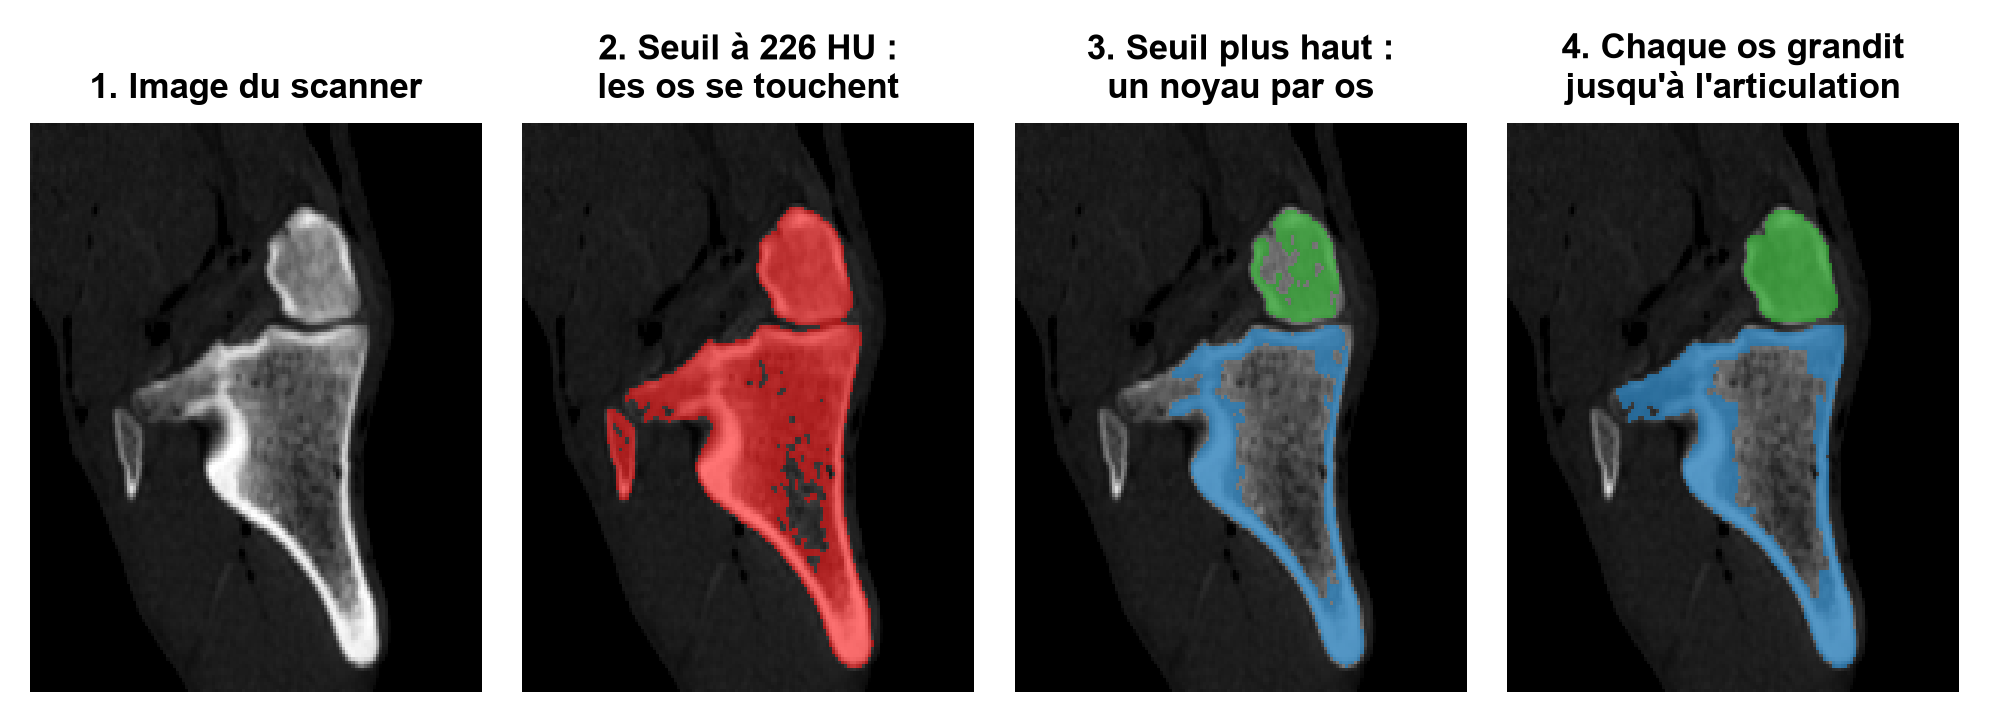
\includegraphics[width=0.85\textwidth]{images/segmentation_principe.png}\par
  \vfill
  {\large Dorian Verstappen, Imane Bikass, Mohamed-Amine Ahmidouch\par}\vspace{0.2cm}
  {Master en ingénierie biomédicale\par ECAM Brussels Engineering School\par}\vspace{0.3cm}
  {\today\par}
\end{center}
\end{titlepage}

\tableofcontents
\clearpage

% ================================================================================================ 1
\section{Introduction}

\subsection{Le problème}

Pour planifier une chirurgie osseuse sur ordinateur, il faut un modèle 3D de l'os du patient. Ce modèle sert à
mesurer des angles, à simuler une coupe et à dessiner des guides de coupe imprimés en 3D qui épousent la surface de
l'os. Le scanner (tomodensitométrie, CT) fournit bien l'information, mais sous une forme qui n'est pas directement
utilisable : un empilement de coupes, c'est-à-dire un grand tableau de nombres. Il ne dit pas où est le fémur, où
commence le tibia, ni quelle est la surface exacte de chaque os.

Ce document décrit comment notre programme passe de ce tableau de nombres à une surface 3D fermée par os. Deux
opérations font l'essentiel du travail :
\begin{itemize}
  \item la \textbf{segmentation} décide, pour chaque petit cube du volume (voxel), à quel os il appartient ;
  \item le \textbf{maillage} transforme chaque os segmenté en une surface faite de triangles, enregistrée dans un
  fichier STL que l'on peut afficher, mesurer ou imprimer.
\end{itemize}

\subsection{Ce que fait le module}

Le module reçoit un dossier de fichiers DICOM (le format des images médicales) et produit, sans aucun clic :
\begin{itemize}
  \item un fichier STL par os reconnu (\fichier{femur.stl}, \fichier{tibia.stl}, \fichier{fibula.stl}\ldots), fermé
  (étanche) et placé dans les coordonnées du scanner, en millimètres ;
  \item un fichier \fichier{segmentation.seg.nrrd} qui contient toutes les étiquettes, avec leurs noms et leurs
  couleurs, lisible par le logiciel libre 3D Slicer \cite{fedorov2012} ;
  \item un rapport (\fichier{rapport.md} et \fichier{rapport.json}) et deux images de contrôle.
\end{itemize}
Pour une série de 750 coupes, le calcul complet prend entre 30 secondes et 2 minutes sur un ordinateur portable.

\subsection{Place dans le projet CT-CORA3D}

CT-CORA3D est un projet de master qui planifie la correction des déformations angulaires des os longs du chien (fémur
et tibia) par la méthode du CORA, puis construit les guides de coupe à imprimer. Le programme est découpé en sept
étapes. Ce document couvre les étapes 1 à 5, qui forment un module indépendant : elles ne savent rien de la chirurgie
et peuvent servir à n'importe quel projet qui a besoin des os d'un scanner en 3D. Les étapes 6 (repères anatomiques)
et 7 (guides de coupe) se contentent de lire les fichiers STL produits ici.

\subsection{Les données utilisées}

Les essais ont été faits sur trois scanners du membre pelvien (patte arrière) d'un lévrier, fournis avec le projet
(\cref{tab-donnees}). Les résultats de ces trois séries sont livrés dans le dossier \fichier{exemples/} du dépôt.

\begin{table}[h]
\centering\small
\caption{Les trois séries du lévrier (scanner GE LightSpeed Ultra, 120~kV, noyau de reconstruction « BONEPLUS »).}
\label{tab-donnees}
\begin{tabular}{llll}
\toprule
\textbf{Série} & \textbf{Région} & \textbf{Coupes × lignes × colonnes} & \textbf{Voxel (mm)} \\
\midrule
\fichier{hip\_to\_knee} (H) & hanche et genou & 728 × 512 × 512 & 0,625 × 0,543 × 0,543 \\
\fichier{knee\_to\_ankle} (G) & genou et cheville & 748 × 512 × 512 & 0,625 × 0,561 × 0,561 \\
\fichier{ankle\_down} (P) & pied & 442 × 512 × 512 & 0,625 × 0,268 × 0,268 \\
\bottomrule
\end{tabular}
\end{table}

\subsection{Les exigences}

Le cahier des charges du projet fixe les exigences suivantes pour cette partie :
\begin{itemize}
  \item des coupes de 1~mm ou moins (au-delà, le programme continue mais avertit) ;
  \item une surface qui coïncide avec la surface réelle de l'os à moins de 0,5~mm ;
  \item un résultat peu sensible au seuil choisi : on fait varier le seuil de ± 50~HU et on mesure l'effet ;
  \item des maillages fermés (imprimables) et exprimés dans les coordonnées du scanner ;
  \item des fichiers relisibles par 3D Slicer, pour vérifier ou retoucher le résultat à la main.
\end{itemize}

\subsection{Organisation du document}

La \cref{sec-notions} rappelle les notions d'imagerie utiles. La \cref{sec-chaine} donne une vue d'ensemble. Les
sections \ref{sec-lecture} à \ref{sec-controle} décrivent les cinq étapes une à une : ce qu'elles font, pourquoi, avec
quelles formules et quels réglages. La \cref{sec-convergence} passe du STL au calcul par éléments finis : une étude
de convergence du maillage, comme on la ferait dans Abaqus, avec des tétraèdres et des hexaèdres linéaires et
quadratiques. La \cref{sec-limites} discute les limites et les pistes d'amélioration, et la
\cref{sec-utiliser} explique comment lancer le module. Les annexes regroupent les paramètres, les fonctions du code et
un petit glossaire.

% ================================================================================================ 2
\section{Notions de base}
\label{sec-notions}

\subsection{Le scanner et les unités Hounsfield}

Le scanner mesure, en chaque point, l'atténuation $\mu$ des rayons X. Pour que les valeurs soient comparables d'un
appareil à l'autre, on les exprime en \textbf{unités Hounsfield} (HU), une échelle fixée par l'eau et l'air :
\begin{equation}
  \mathrm{HU} = 1000\,\frac{\mu - \mu_{\text{eau}}}{\mu_{\text{eau}} - \mu_{\text{air}}}.
\end{equation}
L'eau vaut donc 0~HU et l'air $-1000$~HU. Les ordres de grandeur utiles sont dans le \cref{tab-hu}. Dans un fichier
DICOM, les pixels sont stockés en entiers ; la valeur en HU s'obtient par
$\mathrm{HU} = \text{valeur stockée} \times \texttt{RescaleSlope} + \texttt{RescaleIntercept}$.

\begin{table}[h]
\centering\small
\caption{Ordres de grandeur des unités Hounsfield.}
\label{tab-hu}
\begin{tabular}{lr}
\toprule
\textbf{Tissu} & \textbf{HU} \\
\midrule
air & $-1000$ \\
graisse & environ $-100$ \\
eau & 0 \\
tissus mous (muscle) & 0 à 80 \\
os spongieux & 250 à 700 \\
os cortical & 1200 à 1500 \\
\bottomrule
\end{tabular}
\end{table}

\subsection{Voxel, flou et bruit}

Le volume est découpé en petits pavés, les \textbf{voxels} (de l'ordre de $0{,}6 \times 0{,}5 \times 0{,}5$~mm ici).
Chaque voxel reçoit une seule valeur. Trois défauts compliquent la segmentation :
\begin{itemize}
  \item l'\textbf{effet de volume partiel} : un voxel à cheval sur l'os et les tissus mous prend une valeur
  intermédiaire ; dans une articulation, l'espace entre deux os (l'interligne, 1 à 2~mm) ne fait que quelques voxels
  et n'est jamais vraiment « vide » ;
  \item le \textbf{flou} : le scanner ne voit pas un bord net mais une transition progressive, de l'ordre d'un
  demi-millimètre (sa fonction d'étalement du point) ;
  \item le \textbf{bruit} : des variations aléatoires d'environ 49~HU (écart-type mesuré dans les tissus mous du
  lévrier).
\end{itemize}

\subsection{Le repère du scanner}

Les positions sont données dans le repère du patient appelé \textbf{LPS} : l'axe $x$ va vers la gauche (\emph{Left})
du patient, $y$ vers l'arrière (\emph{Posterior}) et $z$ vers la tête (\emph{Superior}). C'est le repère de la norme
DICOM. Le logiciel 3D Slicer affiche en \textbf{RAS} ($x$ vers la droite, $y$ vers l'avant) : on passe de l'un à
l'autre en changeant le signe de $x$ et de $y$.

Un voxel est repéré par trois indices : $k$ (numéro de coupe), $j$ (ligne) et $i$ (colonne). Une matrice $4 \times 4$
$\vb{A}$ fait le passage des indices aux millimètres :
\begin{equation}
  \begin{pmatrix} x \\ y \\ z \\ 1 \end{pmatrix}
  = \vb{A} \begin{pmatrix} i \\ j \\ k \\ 1 \end{pmatrix},
  \qquad
  \vb{A} = \begin{pmatrix} \Delta_c\,\vb{u}_{\text{ligne}} & \Delta_l\,\vb{u}_{\text{colonne}} & \vb{p}_{\text{pas}} & \vb{o} \\ 0 & 0 & 0 & 1 \end{pmatrix}.
  \label{eq-affine}
\end{equation}
Les vecteurs $\vb{u}$ sont les directions des lignes et des colonnes de l'image (balise DICOM
\texttt{ImageOrientationPatient}), $\Delta_l$ et $\Delta_c$ les tailles des pixels (\texttt{PixelSpacing}),
$\vb{p}_{\text{pas}}$ le déplacement d'une coupe à la suivante et $\vb{o}$ la position du premier voxel
(\texttt{ImagePositionPatient} de la première coupe). Toutes les étapes utilisent cette même matrice : un point
calculé à l'étape 2 tombe donc exactement au même endroit dans le STL de l'étape 4.

\subsection{Segmentation et maillage}

\begin{itemize}
  \item Une \textbf{segmentation} est un tableau de même taille que le volume, qui contient une \emph{étiquette} par
  voxel : 0 pour « pas d'os », puis 1, 2, 3\ldots{} pour chaque os.
  \item Un \textbf{maillage} est une surface faite de triangles qui partagent leurs sommets. Il est \emph{étanche}
  quand il délimite un volume fermé, sans trou : c'est la condition pour pouvoir l'imprimer ou calculer son volume.
  \item Le format \textbf{STL} enregistre simplement la liste des triangles (trois sommets et une normale chacun).
\end{itemize}

% ================================================================================================ 3
\section{Vue d'ensemble de la chaîne}
\label{sec-chaine}

La \cref{fig-chaine} montre les cinq étapes. Chacune est un fichier Python du dossier \fichier{code\_source/} et ne
dépend que de la précédente. Le \cref{tab-etapes} résume ce qu'elles reçoivent et produisent.

\begin{figure}[h]
  \centering
  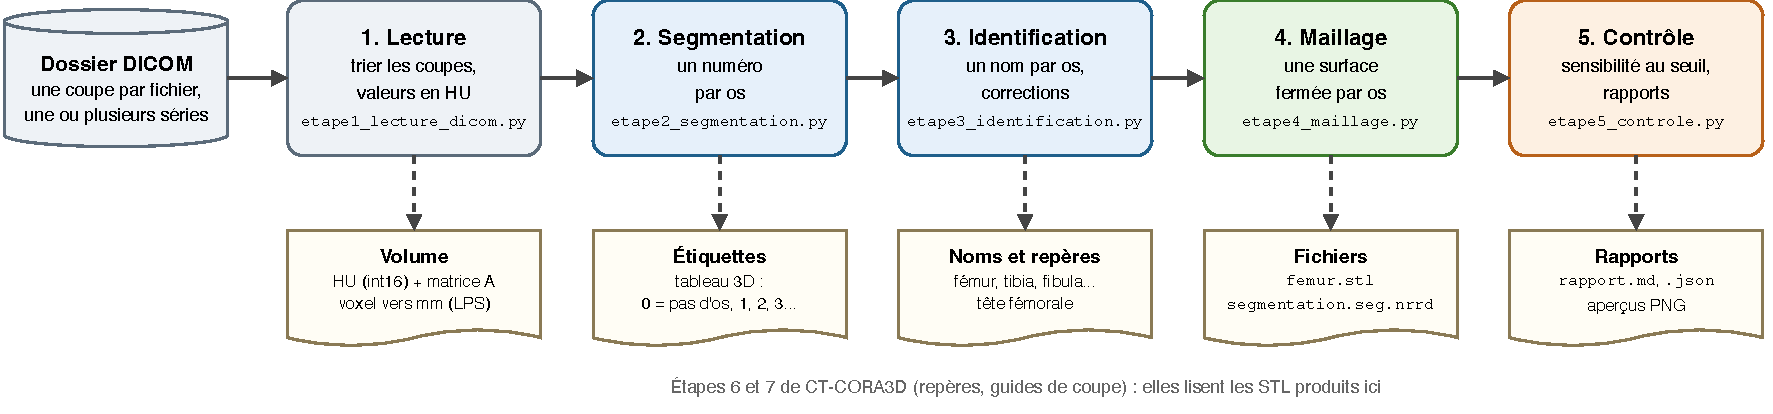
\includegraphics[width=\textwidth]{images/schema_chaine.pdf}
  \caption{Les cinq étapes du module. En haut, le traitement ; en bas, ce que chaque étape transmet à la suivante.}
  \label{fig-chaine}
\end{figure}

\begin{table}[h]
\centering\small
\caption{Les étapes du module, avec leur durée sur la série hanche et genou du lévrier (728 coupes).}
\label{tab-etapes}
\begin{tabularx}{\textwidth}{lYYr}
\toprule
\textbf{Étape} & \textbf{Entrée} & \textbf{Sortie} & \textbf{Durée} \\
\midrule
1. Lecture DICOM & dossier de fichiers & volume en HU et matrice $\vb{A}$ & 10 s \\
2. Segmentation & volume & étiquettes (un numéro par os) & 38 s \\
3. Identification & étiquettes & noms des os, étiquettes corrigées & 20 s \\
4. Maillage & étiquettes nommées & un STL par os, \fichier{segmentation.seg.nrrd} & 25 s \\
5. Contrôle & tout ce qui précède & rapports, aperçus, sensibilité au seuil & 25 s \\
\bottomrule
\end{tabularx}
\end{table}

Les durées des étapes 1, 3, 4 et 5 sont des ordres de grandeur ; celle de l'étape 2 est mesurée par le programme
(lissage 7~s, graines 10,5~s, croissance 15~s, recollage 5~s). Pour les séries genou et cheville et pied, qui sont
bien recadrées, la segmentation ne prend que 8~s et la chaîne entière environ 30~s.

% ================================================================================================ 4
\section{Étape 1 : lire le DICOM}
\label{sec-lecture}

Cette étape est classique mais demande du soin, car une erreur de géométrie fausserait tout le reste sans que rien ne
le signale. Le programme imite le module « DICOM » de 3D Slicer.

\begin{enumerate}
  \item \textbf{Inventaire.} Tous les fichiers du dossier (sous-dossiers compris, extension quelconque) sont ouverts
  sans lire les pixels. Ils sont regroupés par série grâce à l'identifiant unique \texttt{SeriesInstanceUID}. Les
  fichiers qui ne sont pas des images en coupe (rapports, DICOMDIR) sont ignorés.
  \item \textbf{Une seule orientation.} Les images de repérage (« scout ») ont une autre orientation : on garde
  l'orientation la plus fréquente, à $10^{-3}$ près.
  \item \textbf{Tri des coupes.} Les coupes sont triées par leur position le long de la normale à leur plan,
  $d = \vb{o}_{\text{coupe}} \cdot \vb{n}$ avec $\vb{n} = \vb{u}_{\text{ligne}} \times \vb{u}_{\text{colonne}}$, et non par
  leur numéro, qui n'est pas fiable. Les coupes en double sont écartées.
  \item \textbf{Espacement régulier.} Si l'écart entre deux coupes s'éloigne de plus de 5~\% de la médiane (coupe
  manquante), le volume est rééchantillonné par interpolation linéaire sur une grille régulière.
  \item \textbf{Inclinaison du statif.} Si le pas entre coupes n'est pas parallèle à la normale, l'angle est signalé
  et la matrice $\vb{A}$ en tient compte exactement (colonne $\vb{p}_{\text{pas}}$).
  \item \textbf{Valeurs en HU} par la pente et l'ordonnée DICOM, stockées en entiers sur 16 bits ; matrice $\vb{A}$
  (\cref{eq-affine}).
  \item \textbf{Épaisseur.} Des coupes de plus de 1~mm donnent un avertissement.
\end{enumerate}

% ================================================================================================ 5
\section{Étape 2 : séparer les os}
\label{sec-segmentation}

\subsection{La difficulté : les os se touchent}

Un simple seuil ne suffit pas. Au seuil de l'os (226~HU), tout le membre forme un seul bloc : dans chaque
articulation, quelques voxels de volume partiel relient les deux os (\cref{fig-principe}, image 2). Monter le seuil
sépare les os, mais efface aussi l'os spongieux et les corticales fines. L'idée de la méthode est d'utiliser
\textbf{deux seuils} : un seuil haut pour trouver une \emph{graine} par os, puis le seuil bas pour reconstruire chaque
os en entier. La \cref{fig-algo-seg} résume l'algorithme.

\begin{figure}[h]
  \centering
  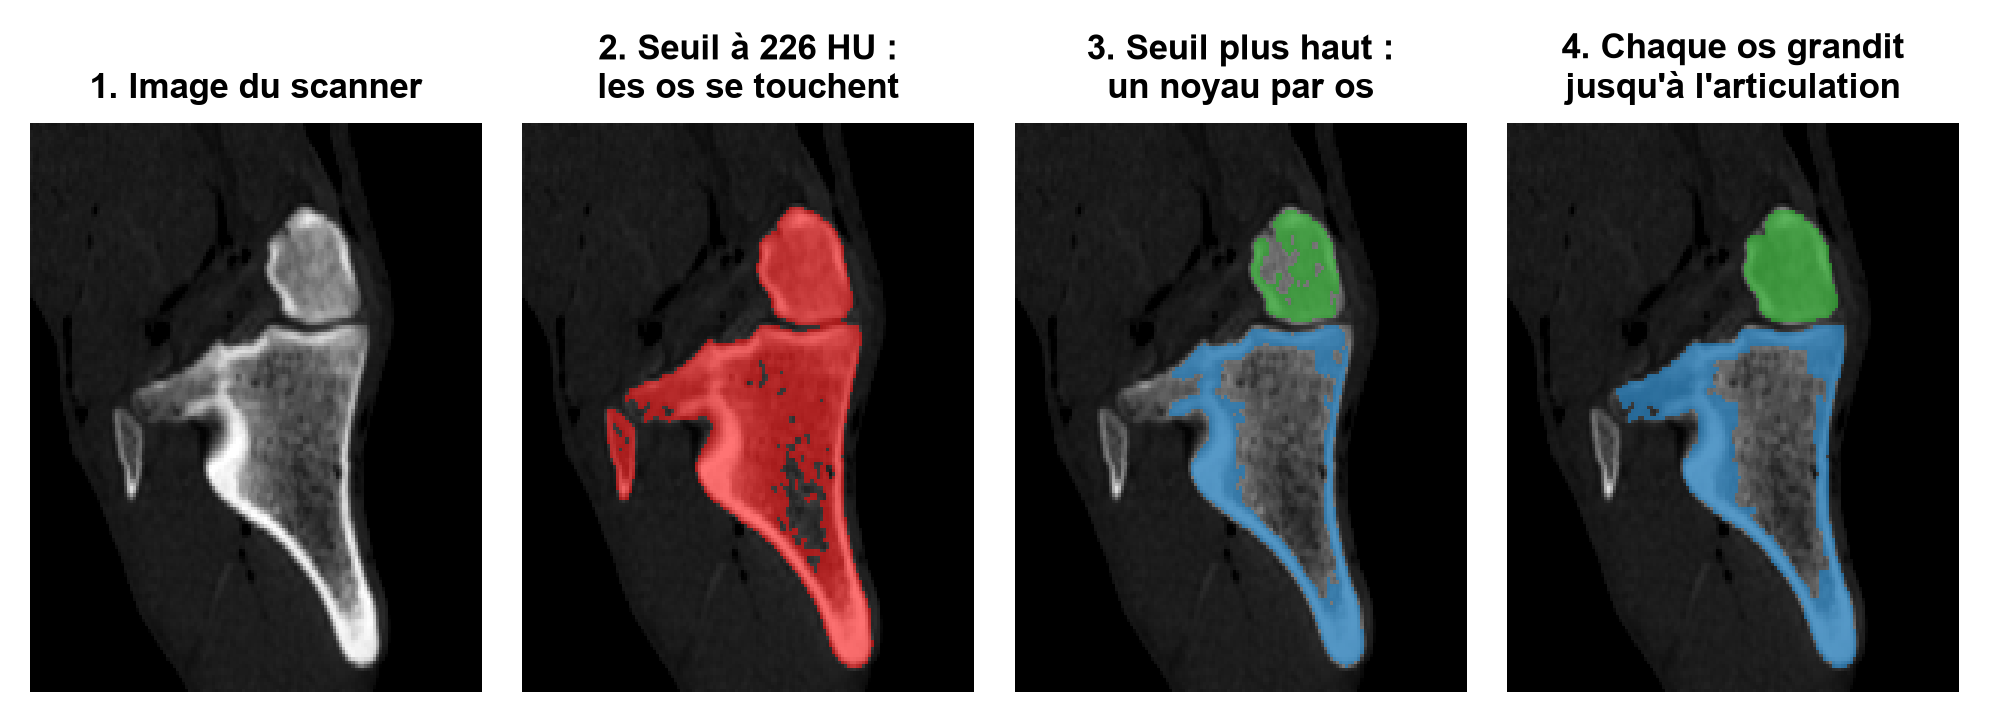
\includegraphics[width=\textwidth]{images/segmentation_principe.png}
  \caption{La segmentation sur une vraie coupe du genou du lévrier : (1) l'image du scanner ; (2) au seuil de
  226~HU, les os se touchent ; (3) avec un seuil plus haut, il reste un noyau par os ; (4) chaque os grandit
  jusqu'à l'articulation. La figure est en 2D ; le programme travaille en 3D.}
  \label{fig-principe}
\end{figure}

\begin{figure}[p]
  \centering
  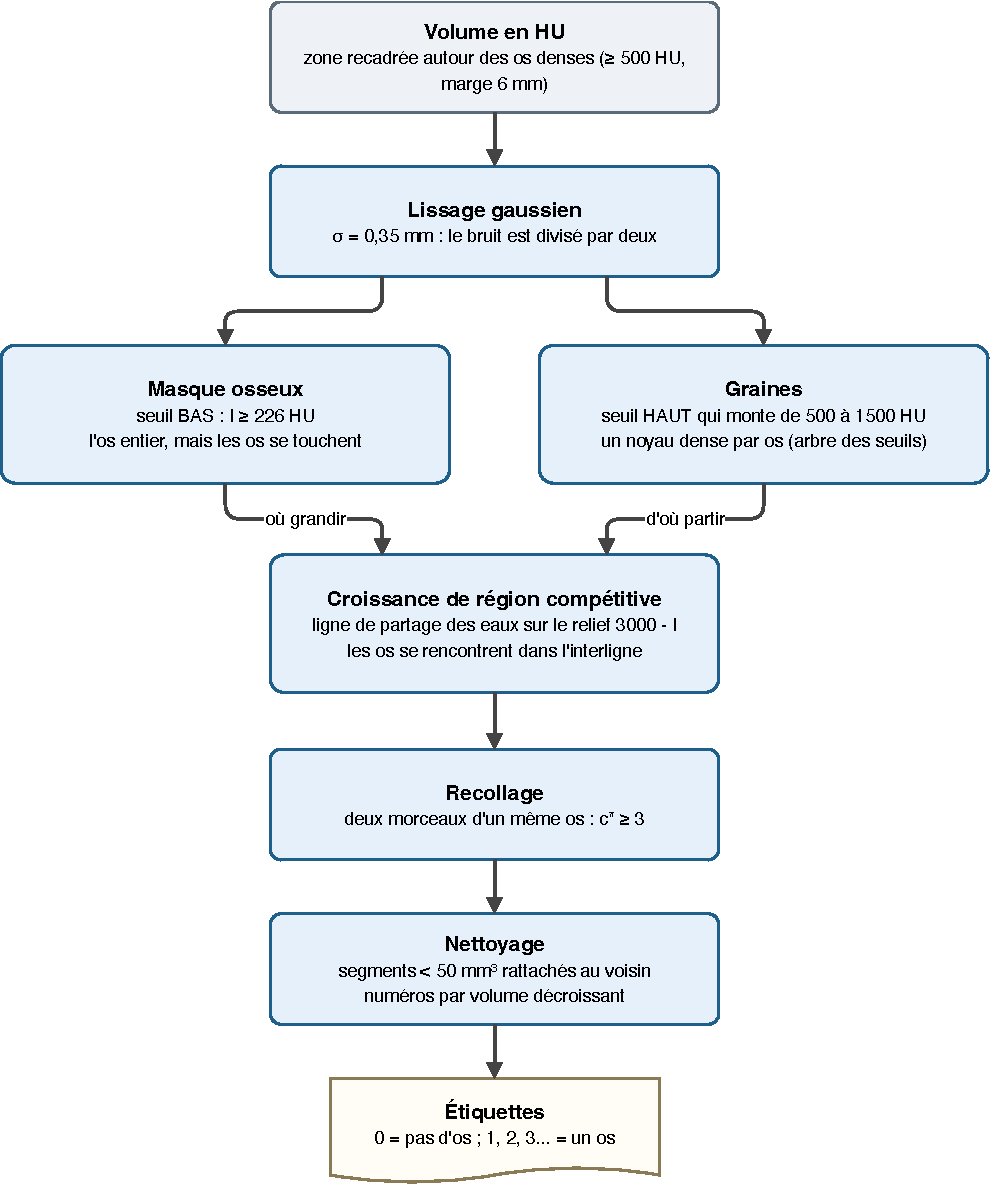
\includegraphics[width=0.78\textwidth]{images/schema_segmentation.pdf}
  \caption{L'algorithme de segmentation (fichier \fichier{etape2\_segmentation.py}, fonction \texttt{segmenter}).}
  \label{fig-algo-seg}
\end{figure}

\subsection{Préparer le volume}

\subsubsection{Recadrer}

Le volume complet contient la table du scanner, l'air et les tissus mous. Le programme cherche d'abord la boîte qui
contient les os denses ($\geq 500$~HU, morceaux d'au moins 30~mm³), en travaillant sur un volume deux fois plus petit
dans chaque direction (un voxel sur deux), puis l'agrandit de 6~mm. Toute la suite se fait dans cette boîte : sur la
série genou et cheville, elle ne fait que 30~\% du volume et la mémoire nécessaire est divisée par cinq environ.

\subsubsection{Lisser}

Le bruit crée des voxels isolés au-dessus du seuil. On applique un flou gaussien de $\sigma = 0{,}35$~mm : chaque
valeur est remplacée par une moyenne pondérée de ses voisines,
\begin{equation}
  I_\sigma(\vb{x}) = \int I(\vb{y})\, \frac{1}{(2\pi\sigma^2)^{3/2}} \exp\!\left(-\frac{\norm{\vb{x}-\vb{y}}^2}{2\sigma^2}\right) \mathrm{d}\vb{y}.
\end{equation}
Le $\sigma$ est donné en millimètres, donc le flou est le même dans les trois directions même si les voxels ne sont
pas cubiques. Ce lissage divise le bruit environ par deux sans effacer les interlignes (1~mm et plus). Il est fait par
le filtre \texttt{SmoothingRecursiveGaussian} de SimpleITK \cite{lowekamp2013}.

\subsubsection{Le masque osseux}

Le masque osseux est l'ensemble $M = \{\vb{x} : I_\sigma(\vb{x}) \geq 226~\mathrm{HU}\}$. Ce seuil est celui que
propose le logiciel commercial Mimics pour l'os au scanner ; le document de cadrage du projet donnait 200 à 300~HU.
C'est un seuil volontairement bas : il garde l'os spongieux et les corticales fines. Nous verrons à la
\cref{sec-demi-hauteur} qu'il place la surface un peu trop à l'extérieur, et comment on corrige ce biais.

\subsection{Une graine par os : le seuil qui monte}
\label{sec-graines}

On monte le seuil par paliers de 100~HU, de 500 à 1500~HU. À chaque palier, on regarde les \textbf{composantes
connexes} : les groupes de voxels au-dessus du seuil qui se touchent (par une face, une arête ou un coin, soit 26
voisins). Quand un bloc se coupe en morceaux, c'est en général parce qu'une articulation, moins dense que l'os, vient
de céder.

Un bloc $B$ est coupé au palier $T$ quand, parmi les composantes de $B \cap \{I_\sigma \geq T\}$, au moins deux :
\begin{itemize}
  \item sont assez grosses : au moins 300~mm³ ;
  \item et \textbf{persistent} : elles gardent au moins 50~mm³ au palier $T + 200$~HU.
\end{itemize}
Chaque morceau retenu est alors examiné à son tour aux paliers suivants. On obtient un arbre : le membre se coupe en
segments, qui se recoupent en os. Les feuilles de l'arbre sont les graines.

\begin{Verbatim}[label={\small Principe de la recherche des graines (pseudo-code)}]
fonction couper(bloc, seuil_courant):
    pour chaque palier T > seuil_courant (de 100 en 100 jusqu'à 1500 HU):
        morceaux = composantes connexes de (bloc ET image >= T)
        retenus  = morceaux d'au moins 300 mm³
                   qui gardent au moins 50 mm³ au-dessus de T + 200 HU
        si au moins 2 retenus:
            renvoyer la réunion des couper(m, T) pour chaque m retenu
    renvoyer [bloc]          # plus de coupure : c'est une graine
\end{Verbatim}

\textbf{Pourquoi la persistance ?} Un vrai os a une corticale dense, qui reste visible quand le seuil monte encore. Un
fragment d'os spongieux, lui, disparaît vite. Sans ce critère, l'épiphyse spongieuse d'un os pourrait devenir une graine
à part.

\textbf{Exemple.} Sur le lévrier, le genou se sépare dès 600~HU, la hanche vers 900~HU (la tête du fémur reste
collée au bassin plus longtemps) et les os du tarse vers 1200 à 1400~HU. La série genou et cheville donne 25 graines.

\subsection{La croissance de région compétitive}
\label{sec-croissance}

Les graines grandissent ensuite toutes en même temps dans le masque osseux $M$. On utilise pour cela la \textbf{ligne
de partage des eaux à partir de marqueurs} (\emph{watershed}) \cite{meyer1994}. On imagine l'image comme un relief :
\begin{equation}
  R(\vb{x}) = \min\bigl(\max\bigl(3000 - I_\sigma(\vb{x}),\ 0\bigr),\ 4500\bigr).
\end{equation}
Les zones denses sont des vallées, les interlignes (peu denses) sont des crêtes. Chaque graine est une source d'eau.
L'eau monte : à chaque instant, on inonde le voxel le plus bas (le plus dense) parmi ceux qui touchent une zone déjà
inondée, et il prend la couleur de cette zone. Deux os qui grandissent se rencontrent donc là où la densité est la
plus faible entre eux, c'est-à-dire dans l'interligne.

\begin{Verbatim}[label={\small Principe de la croissance compétitive (pseudo-code)}]
file = voisins des graines, classés par relief croissant
tant que la file n'est pas vide:
    x = voxel de plus petit relief dans la file
    etiquette[x] = etiquette du voisin déjà inondé qui l'a atteint
    ajouter à la file les voisins de x qui sont dans le masque et pas encore inondés
\end{Verbatim}

Le « fond » (tout ce qui est hors du masque) est aussi une source : il empêche les os de déborder du masque. Le calcul
est fait par la fonction \texttt{MorphologicalWatershedFromMarkers} de SimpleITK.

\textbf{Pourquoi pas une simple croissance de région ?} Une croissance classique ajoute les voisins tant qu'ils sont
au-dessus du seuil. Partie du fémur, elle traverserait le pont de volume partiel du genou et envahirait le tibia. Ici,
les os grandissent \emph{ensemble} et le tibia, parti de sa propre graine, occupe déjà sa place quand le fémur arrive à
l'interligne.

\subsection{Recoller les morceaux d'un même os}
\label{sec-cstar}

À haut seuil, une épiphyse se détache parfois de la diaphyse, parce que la corticale de la métaphyse est fine : un
même os donne alors deux graines. Mais ces deux morceaux se touchent sur \emph{toute la section} de l'os, alors que
deux os voisins ne se touchent que sur une petite surface d'articulation. On mesure cela par un nombre sans
dimension :
\begin{equation}
  \boxed{\;c^* = \frac{A_{\text{contact}}}{V_{\min}^{2/3}}\;}
  \label{eq-cstar}
\end{equation}
où $A_{\text{contact}}$ est la surface de contact entre les deux morceaux (le nombre de faces de voxels qu'ils
partagent, multiplié par l'aire d'une face) et $V_{\min}$ le volume du plus petit des deux.

\textbf{Pourquoi la puissance 2/3 ?} Pour un objet de taille $L$, le volume varie comme $L^3$ et une section comme
$L^2$, donc comme $V^{2/3}$. Le rapport $c^*$ ne dépend donc pas de la taille du chien.

\begin{figure}[h]
  \centering
  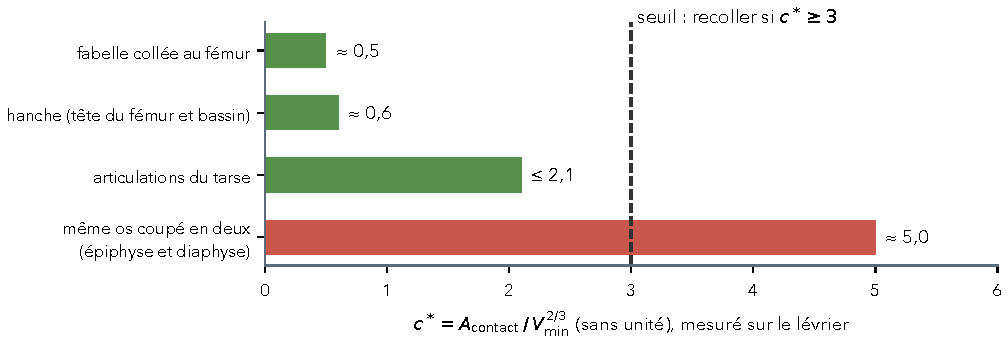
\includegraphics[width=0.92\textwidth]{images/critere_contact.pdf}
  \caption{Le critère $c^*$ mesuré sur le lévrier : les vraies articulations restent sous 2,1 ; un même os coupé en
  deux donne environ 5. Le seuil de recollage est fixé à 3.}
  \label{fig-cstar}
\end{figure}

Le recollage est \emph{glouton} : on fusionne d'abord la paire de plus grand $c^*$, puis on met à jour la table des
contacts sans tout recalculer, grâce à la relation exacte
$A_{\text{contact}}(A \cup B, C) = A_{\text{contact}}(A, C) + A_{\text{contact}}(B, C)$. On recommence tant qu'une paire
dépasse le seuil. Sur la série genou et cheville, deux morceaux sont ainsi recollés ($c^* = 5{,}3$ et $6{,}1$).

\subsection{Nettoyer}

Les segments de moins de 50~mm³ sont rattachés au voisin avec lequel ils ont le plus grand contact, ou supprimés
s'ils sont isolés. Les étiquettes sont ensuite renumérotées par volume décroissant : l'étiquette 1 est le plus gros
os. À ce stade, les os ont un numéro mais pas encore de nom.

\aretenir{la segmentation utilise deux seuils. Le seuil haut (500 à 1500~HU) donne une graine par os ; le seuil bas
(226~HU) dit jusqu'où chaque os peut grandir. La croissance compétitive place la frontière entre deux os dans la zone
la moins dense, l'interligne. Le critère $c^* \geq 3$ recolle les morceaux d'un même os.}

% ================================================================================================ 6
\section{Étape 3 : nommer les os et corriger la segmentation}
\label{sec-identification}

Les étiquettes de l'étape 2 sont anonymes. L'étape 3 leur donne un nom (fémur, tibia\ldots) à partir de leur forme et
de leurs voisins, et en profite pour corriger les erreurs typiques de l'étape 2 : la tête du fémur collée au bassin,
la fibula collée au tibia, une fabelle collée au fémur.

\subsection{Décrire chaque segment}

Pour chaque étiquette, le programme calcule quelques descripteurs simples :
\begin{itemize}
  \item le \textbf{volume} (nombre de voxels × volume d'un voxel) ;
  \item les \textbf{axes principaux}, par une analyse en composantes principales (ACP) des positions des voxels : on
  centre les points, on calcule la décomposition en valeurs singulières, et les vecteurs propres donnent les directions
  de l'os. La \textbf{longueur} $L_1$ est l'étendue le long du premier axe (entre le 1\textsuperscript{er} et le
  99\textsuperscript{e} centile, pour ignorer quelques voxels égarés) ; l'\textbf{allongement} est $L_1 / L_2$ ;
  \item les deux \textbf{extrémités} (moyenne des 5~\% de voxels les plus loin de chaque côté) ;
  \item la \textbf{densité} : HU moyen, coefficient de variation (écart-type divisé par la moyenne) et fraction de voxels
  sous 600~HU (os spongieux), mesurés à l'intérieur du segment pour éviter les bords flous ;
  \item les \textbf{contacts} avec les autres segments (surfaces en mm²) et le contact avec le bord du volume (un os
  coupé par le champ du scanner).
\end{itemize}

\subsection{Écarter les objets qui ne sont pas des os}

Un fantôme de calibration (un cylindre de densité connue posé à côté de l'animal) est dense comme de l'os. On le
reconnaît à son intérieur homogène (coefficient de variation < 0,2, moins de 8~\% de voxels sous 600~HU) et à
l'absence de cavité : quand on le remplit (voir la \cref{sec-remplir}), son volume augmente de moins de 5~\%, alors
qu'un fémur gagne 29~\% (canal médullaire). Sur les séries genou et cheville et pied du lévrier, un cylindre de
1290~HU est ainsi reconnu comme « objet non osseux ».

\subsection{Les règles anatomiques}

Les os sont ensuite reconnus dans un ordre fixé, chaque règle ne s'appliquant qu'aux segments encore sans nom
(\cref{tab-regles}). Un os long est un segment d'au moins 50~mm de long et d'allongement au moins 3.

\begin{table}[h]
\centering\small
\caption{Règles de reconnaissance du membre pelvien, dans l'ordre où elles sont appliquées.}
\label{tab-regles}
\begin{tabularx}{\textwidth}{lY}
\toprule
\textbf{Os} & \textbf{Règle} \\
\midrule
tibia et fibula & os long longé par un os long fin (allongement ≥ 6, moins d'un quart du volume, axes à moins de
20°, côte à côte sur au moins la moitié de la longueur) \\
fémur et bassin & os long dont une extrémité porte une sphère (la tête du fémur) au contact d'un gros os, le bassin
(\cref{sec-tete}) \\
genou & le gros os au contact de l'extrémité la plus large du tibia (le plateau tibial) est le fémur, et inversement \\
fibula collée & petite tache séparée du tibia sur des tranches perpendiculaires à l'os (\cref{sec-fibula}) \\
métatarses & au moins 3 os longs, fins et parallèles, proches les uns des autres \\
tarse & os compacts (allongement < 3,5) reliés de proche en proche au bout du tibia ; le talus a le plus grand
contact avec le tibia, le calcanéus est nettement le plus long \\
phalanges & os au-delà des métatarses \\
patella et fabelles & petits os compacts au contact du fémur (0,5 à 10~\% de son volume) ; le plus gros est la
patella \\
bassin & gros os reliés de proche en proche à l'acétabulum par de larges contacts (≥ 100~mm²) \\
côtés & s'il y a deux fémurs ou deux tibias, chaque os reçoit « gauche » ou « droit » selon sa coordonnée $x$ (LPS) \\
\bottomrule
\end{tabularx}
\end{table}

Le code contient aussi des règles pour la patte avant (humérus, radius, ulna, scapula, carpe), qui ne sont pas
détaillées ici. Les segments qui ne répondent à aucune règle (vertèbres, petits os, débris) restent sans nom : ils
sont gardés dans \fichier{segmentation.seg.nrrd} mais n'ont pas de STL.

\subsection{La tête du fémur : une sphère dans l'interligne}
\label{sec-tete}

La hanche est l'articulation la plus serrée : la tête du fémur est emboîtée dans l'acétabulum, et l'étape 2 la laisse
souvent du côté du bassin. Comme la tête est presque sphérique, on la retrouve en ajustant une sphère sur
l'interligne.
\begin{enumerate}
  \item \textbf{Trouver l'interligne.} L'interligne est une vallée sombre et étroite entre deux zones denses. Le
  « chapeau haut-de-forme noir » (\emph{black top-hat}) la fait ressortir : on applique une fermeture morphologique en
  niveaux de gris de rayon 1~mm (qui comble les vallées étroites), puis on soustrait l'image. Les voxels où la
  différence dépasse 250~HU, et dont la densité reste au-dessus de 150~HU (pour écarter les cloisons de graisse entre
  les muscles), sont les points candidats.
  \item \textbf{Ajuster une sphère par RANSAC} \cite{fischler1981}. Une sphère de centre $\vb{c}$ et de rayon $r$
  vérifie $\norm{\vb{x}}^2 = 2\,\vb{c}\cdot\vb{x} + (r^2 - \norm{\vb{c}}^2)$, une équation \emph{linéaire} en
  $(\vb{c}, r^2 - \norm{\vb{c}}^2)$. Quatre points tirés au hasard donnent donc une sphère par un simple système
  $4 \times 4$. On répète 4000 fois et on garde la sphère qui a le plus de points à moins de 0,6~mm de sa surface,
  puis on l'affine par moindres carrés sur ces points.
  \item \textbf{Vérifier.} La sphère est acceptée si son rayon est plausible (4 à 20~mm), si elle a au moins 150
  points, si ces points couvrent au moins 40~\% des directions autour du centre, et si le rayon reste petit devant la
  longueur de l'os (moins de 9~\%). Un os qui porte des dents (émail au-dessus de 2250~HU) n'est jamais un fémur :
  ce garde-fou évite de confondre une mandibule articulée au crâne avec une hanche.
  \item \textbf{Redistribuer.} Les deux segments sont refaits par une nouvelle croissance compétitive : graine
  « fémur » = intérieur de la sphère (rayon moins 1~mm) plus la diaphyse ; graine « bassin » = tout ce qui est au-delà
  de la sphère (rayon plus 1~mm).
\end{enumerate}

\textbf{Exemple.} Série hanche et genou : sphère de rayon 12,6~mm ajustée sur 2055 points de l'interligne, qui
couvrent 69~\% des directions.

\subsection{La fibula collée au tibia}
\label{sec-fibula}

La fibula est fine et touche le tibia à ses deux extrémités : elle peut ne pas avoir sa propre graine. Le programme
coupe alors le segment « tibia » en tranches de 2~mm perpendiculaires à son axe. Au milieu de la jambe, la fibula
apparaît sur chaque tranche comme une petite tache séparée (aire au moins 3~mm², moins de 20~\% de l'aire du tibia).
Si cette petite tache existe sur une suite de tranches couvrant au moins 15~\% de la longueur, et se déplace de moins
de 3~mm d'une tranche à l'autre, ses voxels deviennent la graine « fibula » et ceux des grandes taches la graine
« tibia ». Une nouvelle croissance compétitive redistribue le segment. Le résultat est annulé s'il est invraisemblable
(fibula de moins de 2~\% ou de plus de 25~\% du volume du tibia, ou trop courte).

\textbf{Exemple.} Série genou et cheville : fibula vue séparée sur 106~mm (44~\% de la longueur), 4,9~cm³.

\subsection{Les outils de correction}

Plusieurs outils de l'étape 2 sont réutilisés ici, et par l'application quand l'utilisateur corrige à la main :
\begin{itemize}
  \item \textbf{nouvelle croissance} (\texttt{recroissance}) : une zone (une ou plusieurs étiquettes) est entièrement
  redistribuée à partir de graines imposées ; c'est elle qui sépare tête du fémur et bassin, tibia et fibula ;
  \item \textbf{raffinement} (\texttt{raffiner}) : on cherche des graines plus fines (taille minimale et persistance
  divisées par 2 ou 3) dans un seul segment. Il détache par exemple une fabelle (petit os sésamoïde derrière le genou)
  collée au fémur : un morceau de moins de 5~\% du fémur, compact, et peu en contact ($c^* < 1{,}5$) devient une
  fabelle ; tout autre morceau est rendu au fémur ;
  \item \textbf{lissage de frontière} (\texttt{lisser\_frontiere}) : un filtre majoritaire près de la frontière de
  deux os supprime les îlots et les « doigts » qu'un os envoie dans son voisin quand l'interligne est trop fin ;
  \item \textbf{points de l'utilisateur} : un fichier \fichier{graines.json} contient des points nommés
  (\cref{sec-graines-json}). Un point seul dans un segment le renomme ; des points de noms différents dans le même
  segment le séparent, par une croissance à partir de boules de 2,5~mm autour des points.
\end{itemize}

Enfin, un os nommé doit être d'un seul tenant : un morceau détaché est rendu au voisin dont il a été découpé s'il le
touche sur toute une section ($c^* \geq 3$), sinon il devient un segment à part.

\aretenir{les noms viennent de règles simples sur la forme (ACP, allongement) et le voisinage (surfaces de contact).
L'étape 3 corrige aussi la segmentation là où l'étape 2 échoue de façon prévisible : la hanche (sphère RANSAC), la
fibula (tranches) et les fabelles (raffinement).}

% ================================================================================================ 7
\section{Étape 4 : fabriquer les surfaces}
\label{sec-maillage}

L'étape 4 transforme chaque os nommé en une surface fermée. Il y a un fichier par os, et des groupes : par exemple
\fichier{tarse.stl} réunit le talus, le calcanéus et les autres os du tarse. La \cref{fig-algo-maillage} montre les
opérations dans l'ordre.

\begin{figure}[h]
  \centering
  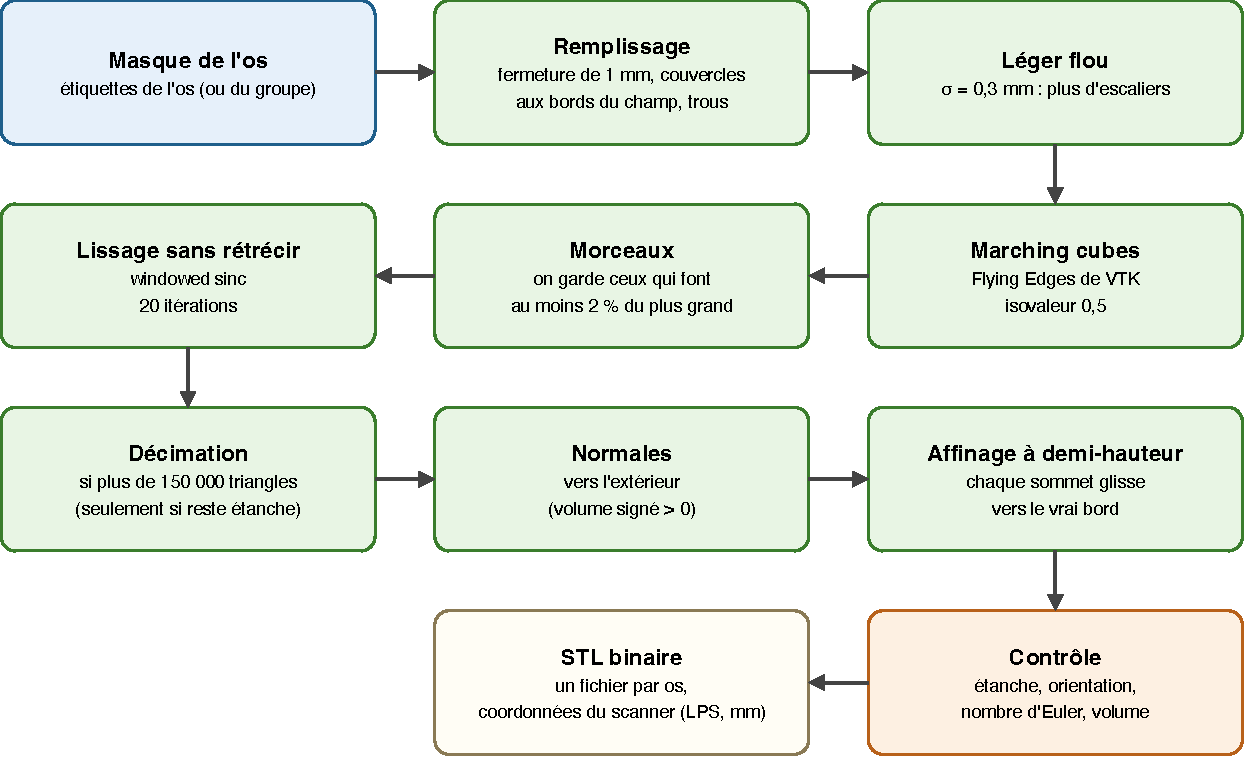
\includegraphics[width=0.95\textwidth]{images/schema_maillage.pdf}
  \caption{Du masque d'un os au fichier STL (fichier \fichier{etape4\_maillage.py}, fonction \texttt{mailler}).}
  \label{fig-algo-maillage}
\end{figure}

\subsection{Remplir l'os}
\label{sec-remplir}

Le STL doit décrire la surface extérieure de l'os, pas le canal médullaire. On remplit donc chaque os :
\begin{enumerate}
  \item une \textbf{fermeture morphologique} de rayon 1~mm (une dilatation suivie d'une érosion) bouche les petits
  pores de la corticale ;
  \item si l'os sort du champ du scanner, sa section au bord est d'abord fermée par un \textbf{couvercle} (la section
  remplie en 2D) : sinon le canal resterait ouvert sur l'extérieur et ne serait pas rempli ;
  \item un \textbf{remplissage des trous} en 3D remplit tout ce qui n'est pas relié à l'extérieur : canal et os
  spongieux.
\end{enumerate}

\subsection{Extraire la surface : marching cubes}

Le masque rempli vaut 1 dans l'os et 0 dehors. On le floute légèrement ($\sigma = 0{,}3$~mm) pour obtenir un champ $g$
qui passe en douceur de 1 à 0, puis on extrait la surface $g = 0{,}5$ par l'algorithme des \textbf{marching cubes}
\cite{lorensen1987}, dans sa version rapide \emph{Flying Edges} de VTK \cite{schroeder2015}.

Le principe : on parcourt les petits cubes formés par 8 voxels voisins. Pour chaque cube, on regarde quels coins sont
au-dessus de 0,5 ; parmi les $2^8 = 256$ cas possibles, une table donne les triangles à placer dans le cube. Un sommet
posé sur l'arête qui relie deux coins $a$ et $b$ est placé par interpolation linéaire :
\begin{equation}
  \vb{x} = \vb{x}_a + t\,(\vb{x}_b - \vb{x}_a), \qquad t = \frac{0{,}5 - g_a}{g_b - g_a}.
\end{equation}
Le léger flou supprime l'effet d'escalier des voxels. Les sommets, calculés en indices de voxels, passent ensuite en
millimètres par la matrice $\vb{A}$ (\cref{eq-affine}).

Si la surface obtenue a plusieurs morceaux, on ne garde que ceux qui ont au moins 2~\% de l'aire du plus grand : les
miettes sont supprimées, mais les os d'un groupe (le tarse, les phalanges) sont tous gardés.

\subsection{Lisser sans rétrécir}

Un lissage simple, qui rapproche chaque sommet de la moyenne de ses voisins (lissage laplacien), fait rétrécir le
maillage à chaque passe. On utilise un lissage « à fenêtre sinc » (\emph{windowed sinc}) \cite{taubin1995} :
c'est un filtre passe-bas sur la position des sommets, qui enlève les petites bosses sans changer la taille de
l'objet. Réglages : 20 itérations, bande passante 0,05. C'est aussi le choix de 3D Slicer.

\subsection{Alléger}

Au-delà de 150\,000 triangles (environ 7~Mo de STL), le maillage est simplifié par la méthode des \textbf{quadriques}
\cite{garland1997}. Chaque sommet accumule une matrice $\vb{Q} = \sum_p \vb{p}\vb{p}^{\mathsf T}$, où
$\vb{p} = (a, b, c, d)$ décrit le plan $ax + by + cz + d = 0$ de chaque triangle voisin. L'erreur
$\vb{x}^{\mathsf T}\vb{Q}\,\vb{x}$ (en coordonnées homogènes) est la somme des carrés des distances de $\vb{x}$ à ces
plans. On fusionne en priorité les paires de sommets dont la fusion coûte le moins. La simplification ne retire jamais
plus de 75~\% des triangles, et elle n'est gardée que si le maillage reste étanche.

\subsection{Orienter les normales}

Les triangles doivent tous être parcourus dans le même sens, de façon que leurs normales sortent de l'os. Le volume
signé du maillage se calcule par
\begin{equation}
  V = \frac{1}{6} \sum_{\text{triangles}} \vb{a}\cdot(\vb{b}\times\vb{c}),
\end{equation}
où $\vb{a}$, $\vb{b}$ et $\vb{c}$ sont les sommets de chaque triangle. Il est positif quand les normales sortent ; s'il
est négatif, on retourne tous les triangles.

\subsection{Placer la surface au vrai bord : l'affinage à demi-hauteur}
\label{sec-demi-hauteur}

\subsubsection{Le biais d'un seuil bas}

Le scanner floute les bords. Modélisons un bord d'os par une marche floutée : du côté de l'os (position $s < 0$ le
long de la normale) l'intensité vaut $C$ (corticale, environ 1300~HU), dehors elle vaut $B$ (tissus mous, environ
40~HU), et entre les deux
\begin{equation}
  I(s) = B + (C - B)\,\Phi\!\left(-\frac{s}{\sigma}\right),
\end{equation}
où $\Phi$ est la fonction de répartition de la loi normale et $\sigma$ l'écart-type du flou. Le vrai bord est en
$s = 0$, là où l'intensité vaut la moitié entre $B$ et $C$. Un seuil $T$ place la surface là où $I(s) = T$, donc en
\begin{equation}
  \boxed{\;s_T = -\sigma\,\Phi^{-1}\!\left(\frac{T - B}{C - B}\right).\;}
  \label{eq-biais}
\end{equation}
Un seuil bas ($T$ proche de $B$) donne $\Phi^{-1} < 0$, donc $s_T > 0$ : la surface est trop à l'extérieur.

\begin{figure}[h]
  \centering
  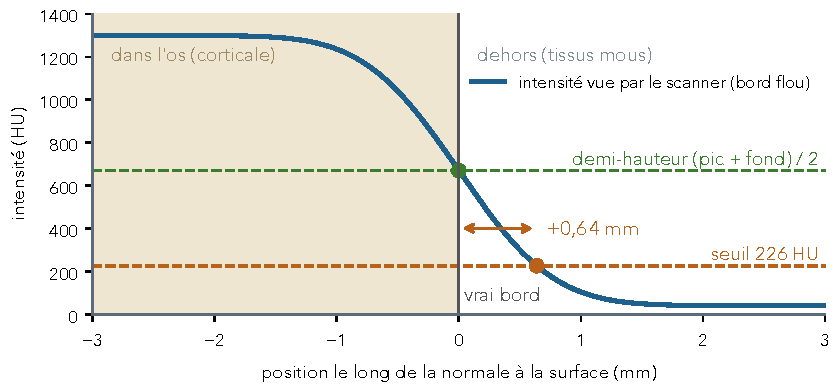
\includegraphics[width=0.92\textwidth]{images/profil_bord.pdf}
  \caption{Un seuil bas (226~HU) place la surface trop à l'extérieur d'environ un écart-type du flou ; la
  demi-hauteur retrouve le vrai bord.}
  \label{fig-profil}
\end{figure}

\textbf{Exemple chiffré.} Fantôme du test automatique (\cref{sec-fantome}) : flou du scanner 0,5~mm et lissage du
programme 0,35~mm, soit $\sigma = \sqrt{0{,}5^2 + 0{,}35^2} = 0{,}61$~mm. Avec $T = 226$, $B = 40$ et $C = 1300$~HU :
$(T - B)/(C - B) = 0{,}148$, $\Phi^{-1}(0{,}148) = -1{,}05$, donc $s_T = +0{,}64$~mm. Le test mesure $+0{,}60$~mm.
C'est plus que la tolérance de 0,5~mm : il faut corriger.

\subsubsection{La correction}

Chaque sommet est déplacé le long de sa normale jusqu'au point où l'intensité vaut la moitié entre le pic de la
corticale et le fond :
\begin{enumerate}
  \item on lit le profil d'intensité le long de la normale, de 2,5~mm à l'intérieur à 2~mm à l'extérieur, tous les
  0,1~mm (interpolation trilinéaire dans l'image lissée) ;
  \item le \emph{pic} est le maximum du côté intérieur, le \emph{fond} le minimum après le pic ;
  \item le nouveau bord est le premier point, après le pic, où le profil passe sous $(\text{pic} + \text{fond})/2$
  (interpolation linéaire entre deux échantillons) ;
  \item le déplacement est ignoré si le contraste est faible (pic moins fond < 300~HU) ou s'il dépasse 1,5~mm
  (articulation serrée, profil douteux) ;
  \item les déplacements sont lissés sur le maillage (cinq passes de moyenne avec les voisins), pour ne pas créer de
  bruit d'un sommet à l'autre ;
  \item le maillage déplacé n'est gardé que s'il reste étanche.
\end{enumerate}

\textbf{Résultat.} Sur le fantôme, l'écart passe de $+0{,}60$ à $+0{,}16$~mm ; le reste vient de la corticale très
fine du fantôme (1,5~mm), dont le pic est atténué par le flou. Sur le lévrier, les sommets reculent en moyenne de 0,21
à 0,32~mm vers l'intérieur selon l'os, et plus de 90~\% des sommets sont affinés.

\subsection{Vérifier que la surface est fermée}
\label{sec-topologie}

Un fichier à imprimer doit décrire un solide fermé. Le programme vérifie, avec la bibliothèque trimesh :
\begin{itemize}
  \item l'\textbf{étanchéité} : chaque arête est partagée par exactement deux triangles ;
  \item l'\textbf{orientation} : deux triangles voisins parcourent leur arête commune en sens opposés ;
  \item la \textbf{caractéristique d'Euler} $\chi = S - A + F$ (sommets, arêtes, faces). Pour une surface fermée faite
  de $n$ morceaux, $\chi = 2n - 2g$, où $g$ est le nombre total de « anses » (trous qui traversent l'objet, comme
  celui d'une tasse). Un os seul sans trou, qui a la forme topologique d'une sphère, doit donner $\chi = 2$.
\end{itemize}

Tous les os seuls du lévrier donnent $\chi = 2$. Pour les groupes, d'autres valeurs sont normales : le bassin donne
$\chi = -58$, car il est fait de plusieurs os soudés qui forment des anneaux (trous obturés, arcs des vertèbres) ; les
métatarses et le tarse donnent 0 (un morceau avec une anse : des os voisins qui se touchent en deux endroits) ; les
phalanges de la série genou et cheville donnent 4 (deux morceaux sans anse). Ces groupes ne servent pas à la
planification.

\subsection{Les fichiers écrits}

\begin{itemize}
  \item \textbf{STL binaire} : 80 octets d'en-tête (nom du programme, version, nom de l'os, repère), le nombre de
  triangles sur 4 octets, puis 50 octets par triangle : sa normale et ses trois sommets (12 réels de 4 octets) et 2
  octets libres. Les coordonnées sont en millimètres, dans le repère LPS du scanner (option RAS possible).
  \item \textbf{\fichier{segmentation.seg.nrrd}} : toutes les étiquettes de la zone recadrée, compressées, avec la
  géométrie (origine et directions) et, pour chaque segment, son nom et sa couleur. Ouvert dans 3D Slicer par-dessus la
  série DICOM, il permet de vérifier la segmentation coupe par coupe et de la retoucher ; le programme sait le relire.
  \item \textbf{Bords du champ} : pour chaque os, le programme note les bords du volume qu'il touche (un plan et sa
  normale). Un os coupé par le champ est incomplet ; l'étape 6 refuse de planifier un tel os.
\end{itemize}

% ================================================================================================ 8
\section{Étape 5 : contrôler et valider}
\label{sec-controle}

\subsection{Un faux scanner dont on connaît tout}
\label{sec-fantome}

On ne connaît pas la vraie surface des os du lévrier. Pour mesurer l'exactitude, le test automatique
\fichier{tests/test\_chaine.py} fabrique un faux scanner dont la géométrie est connue exactement :
\begin{itemize}
  \item deux « os » en forme de capsule (cylindre de 7~mm de rayon à bouts hémisphériques), bout à bout, séparés par
  un interligne de 1,5~mm et inclinés de 15° ;
  \item une corticale de 1,5~mm à 1300~HU, une moelle et des tissus mous à 40~HU ;
  \item une table de scanner (300~HU) et un cylindre de calibration homogène (1300~HU) ;
  \item un flou gaussien de 0,5~mm et un bruit de 40~HU ; voxels de $0{,}625 \times 0{,}5 \times 0{,}5$~mm.
\end{itemize}
Le volume est écrit en vrais fichiers DICOM, aux noms mélangés, puis relu par le programme comme un vrai scanner. Le
test fait 14 vérifications ; toutes passent (\cref{tab-fantome}), en 2 secondes.

\begin{table}[h]
\centering\small
\caption{Résultats du test sur le faux scanner (identiques pour les deux os ; exécution du 23/11/2026).}
\label{tab-fantome}
\begin{tabularx}{\textwidth}{Yl}
\toprule
\textbf{Vérification} & \textbf{Résultat} \\
\midrule
lecture : une série, dimensions, espacement, position LPS d'un voxel connu & exactes \\
segmentation : deux os séparés malgré l'interligne de 1,5~mm & oui \\
le cylindre est reconnu « objet non osseux », la table est ignorée & oui \\
maillage étanche, un morceau, $\chi = 2$ & oui \\
écart moyen à la vraie surface, seuil seul & $+0{,}60$~mm (théorie : $+0{,}64$~mm) \\
écart moyen à la vraie surface, avec affinage à demi-hauteur & $+0{,}16$~mm (95\textsuperscript{e} centile 0,22~mm) \\
volume (vrai : 8,71~cm³) & 10,39~cm³ sans affinage, 9,13~cm³ avec \\
\bottomrule
\end{tabularx}
\end{table}

\subsection{La sensibilité au seuil}
\label{sec-sensibilite}

Le seuil de 226~HU est un choix. Pour vérifier que le résultat n'en dépend pas trop, l'étape 5 refait chaque os
principal à 176 puis à 276~HU, dans la même zone (l'os dilaté de 3~mm, sans les autres os), le remplit de la même façon,
et mesure la distance de chaque sommet de cette nouvelle surface à la surface de référence.

La distance est calculée avec une précision inférieure au voxel. Si $g$ est le masque de référence flouté (celui du
STL) et $\vb{p}$ un point proche de la surface $g = 0{,}5$, un développement au premier ordre donne
\begin{equation}
  g(\vb{p}) \approx 0{,}5 - d\,\norm{\nabla g(\vb{p})}
  \quad\Longrightarrow\quad
  d \approx \frac{0{,}5 - g(\vb{p})}{\norm{\nabla g(\vb{p})}},
\end{equation}
avec $d > 0$ quand la nouvelle surface est à l'extérieur. Loin de la surface ($g$ proche de 0 ou de 1), on prend une
carte de distance exacte au voxel près (transformée de Maurer \cite{maurer2003}).

\begin{figure}[h]
  \centering
  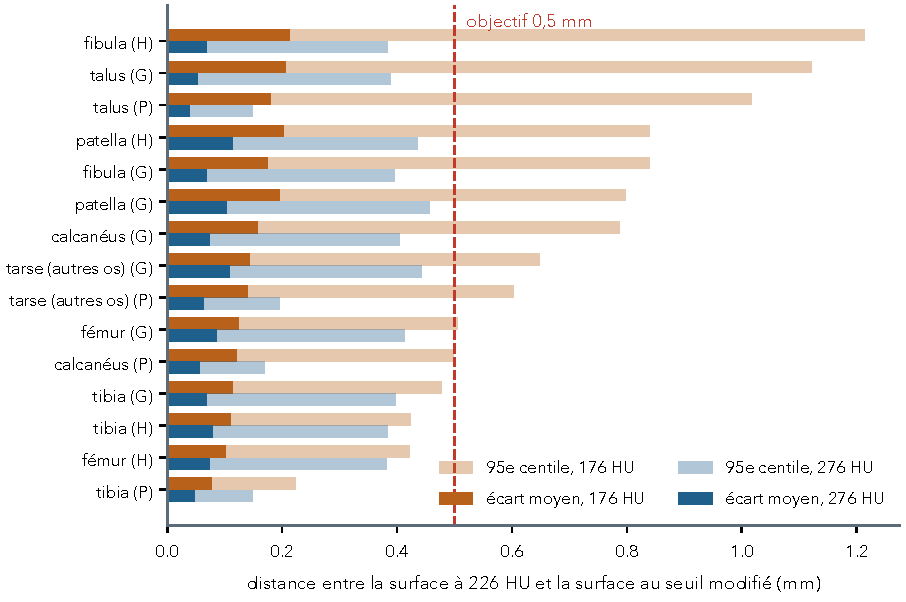
\includegraphics[width=0.95\textwidth]{images/sensibilite.pdf}
  \caption{Écart entre la surface à 226~HU et les surfaces à 176~HU (orange) et 276~HU (bleu), pour chaque os
  contrôlé des trois séries (H : hanche et genou, G : genou et cheville, P : pied). Barre foncée : écart moyen ; barre
  claire : 95\textsuperscript{e} centile.}
  \label{fig-sensibilite}
\end{figure}

\textbf{Lecture des résultats} (\cref{fig-sensibilite}) :
\begin{itemize}
  \item l'écart moyen reste entre 0,04 et 0,21~mm pour tous les os : bien sous l'objectif de 0,5~mm ;
  \item pour les grands os (fémur, tibia), 95~\% des points restent à moins de 0,5~mm, dans les deux sens ;
  \item pour les petits os fins (fibula, talus, patella, calcanéus), baisser le seuil à 176~HU fait bouger quelques
  zones de plus de 0,5~mm (95\textsuperscript{e} centile jusqu'à 1,2~mm pour la fibula de la série H) : à bas seuil,
  le volume partiel des corticales fines et des articulations serrées est pris dans l'os. Le volume de la fibula
  augmente alors de 11~\%, celui du fémur de 1,3~\% seulement ;
  \item monter le seuil à 276~HU est presque sans effet (95\textsuperscript{e} centile ≤ 0,46~mm partout).
\end{itemize}

\subsection{Les résultats sur le lévrier}

Sur les trois séries, sans aucune intervention, le programme reconnaît le fémur, le tibia, la fibula, la patella, les
fabelles, le talus, le calcanéus, les autres os du tarse, les métatarses, les phalanges et le bassin, et écarte le
cylindre de calibration. Tous les maillages sont étanches et correctement orientés (\cref{tab-levrier}).

\begin{table}[h]
\centering\small
\caption{Maillages des os principaux (série G : genou et cheville ; fémur de la série H). Volume du maillage après
affinage ; affinage = déplacement moyen des sommets (négatif : vers l'intérieur).}
\label{tab-levrier}
\begin{tabular}{lrrrrr}
\toprule
\textbf{Os} & \textbf{Volume (cm³)} & \textbf{Triangles} & \textbf{Étanche} & $\boldsymbol{\chi}$ & \textbf{Affinage (mm)} \\
\midrule
fémur (H) & 100,3 & 150\,000 & oui & 2 & $-0{,}23$ \\
tibia & 82,2 & 150\,000 & oui & 2 & $-0{,}24$ \\
fibula & 3,8 & 38\,700 & oui & 2 & $-0{,}26$ \\
patella & 2,2 & 8\,556 & oui & 2 & $-0{,}24$ \\
talus & 5,6 & 21\,308 & oui & 2 & $-0{,}31$ \\
calcanéus & 14,0 & 44\,124 & oui & 2 & $-0{,}28$ \\
fabelles & 0,4 & 3\,028 & oui & 2 & $-0{,}28$ \\
\bottomrule
\end{tabular}
\end{table}

\begin{figure}[h]
  \centering
  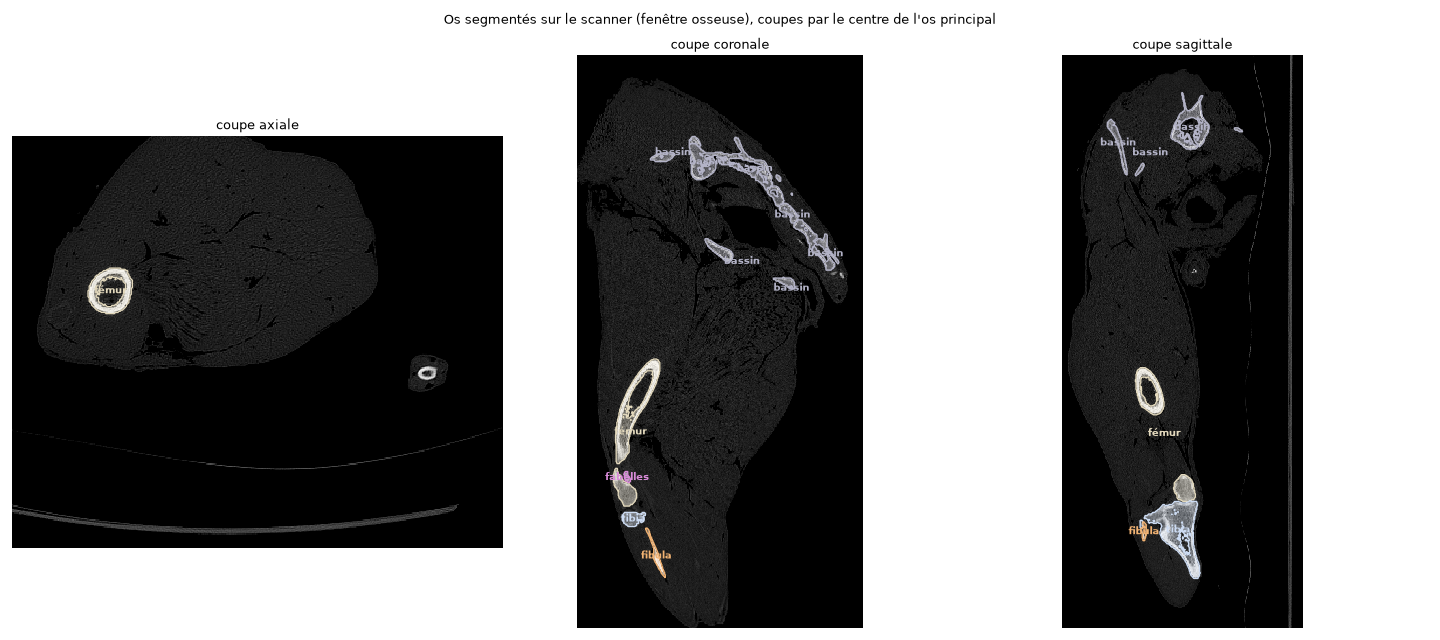
\includegraphics[width=\textwidth]{images/apercu_coupes_hanche_genou.png}
  \caption{Image de contrôle produite par l'étape 5 (série hanche et genou) : trois coupes passant par le centre du
  fémur, avec le contour et le nom de chaque os.}
  \label{fig-coupes}
\end{figure}

\begin{figure}[h]
  \centering
  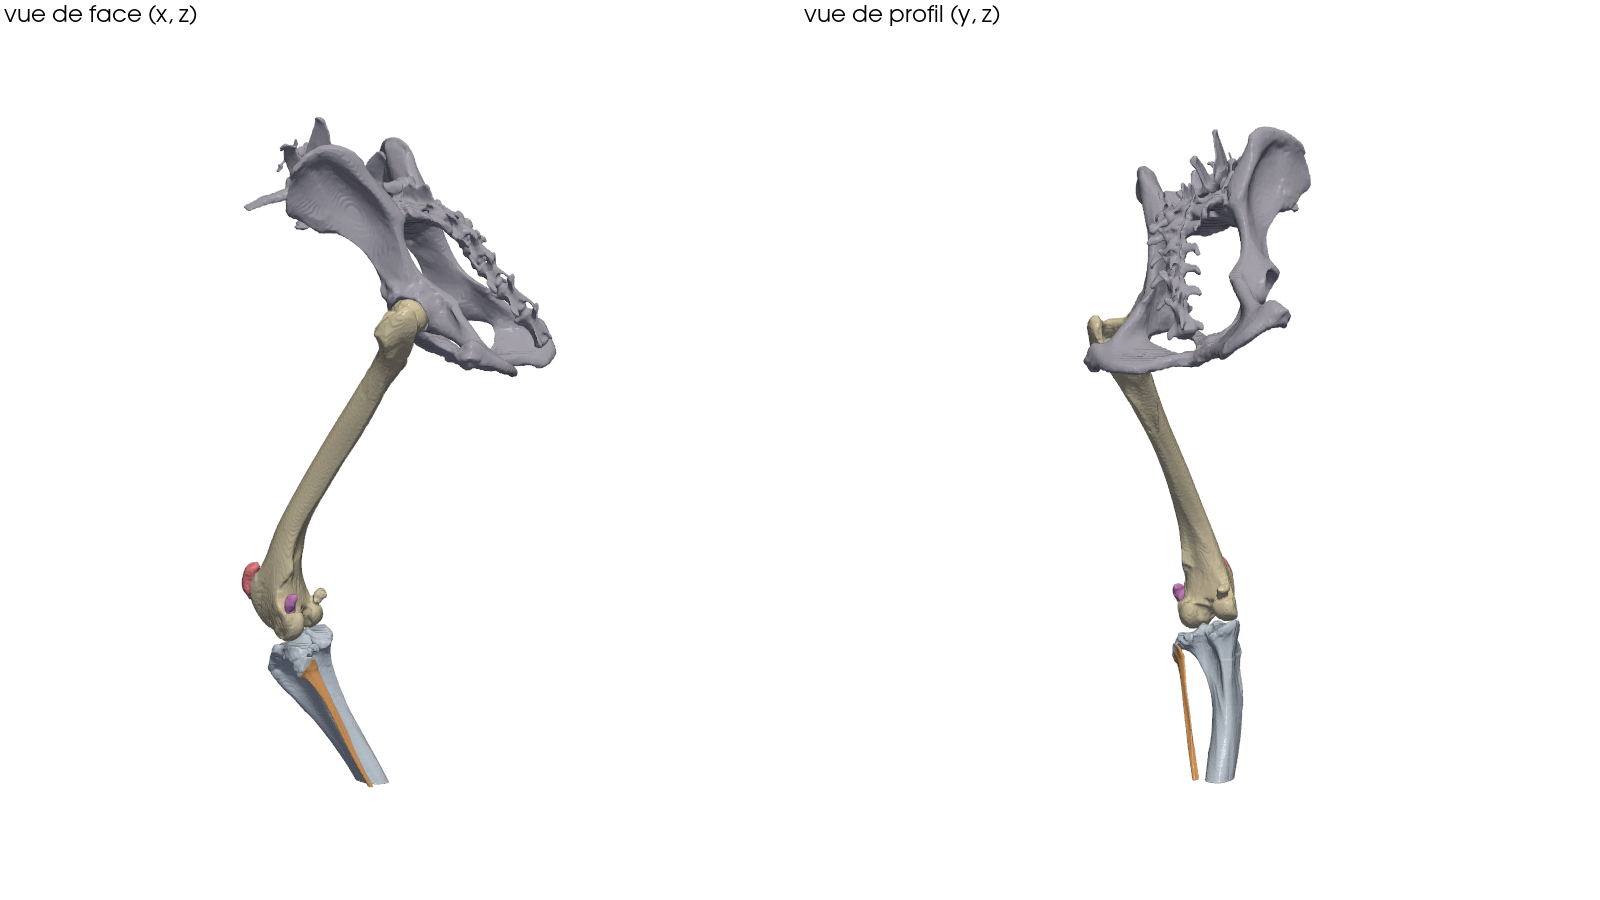
\includegraphics[width=0.75\textwidth]{images/segmentation_resultat.png}
  \caption{Les os segmentés et maillés automatiquement dans le scanner hanche et genou du lévrier.}
  \label{fig-resultat}
\end{figure}

\subsection{Les rapports}

Pour chaque série, l'étape 5 écrit dans \fichier{resultats/<série>/} :
\begin{itemize}
  \item \fichier{rapport.md} (lisible) et \fichier{rapport.json} (toutes les valeurs, y compris tous les paramètres
  utilisés) : la série, les os exportés (volume, triangles, étanchéité, Euler, affinage, sensibilité au seuil),
  l'identification avec la raison de chaque nom, les avertissements ;
  \item \fichier{apercu\_3d.png} et \fichier{apercu\_coupes.png} (\cref{fig-coupes}), pour un contrôle visuel rapide ;
  \item \fichier{reperes\_auto.mrk.json} : le centre de la tête du fémur, au format « Markups » de 3D Slicer.
\end{itemize}
Remarque : les rapports recopient le nom du patient et son identifiant lus dans l'en-tête DICOM. Il vaut mieux
anonymiser les dossiers avant de partager ces fichiers.

% ================================================================================================ 8 bis
\section{Du STL au calcul par éléments finis : étude de convergence}
\label{sec-convergence}

Le STL de l'étape 4 décrit la \emph{surface} de l'os. Pour calculer des contraintes (par exemple avec Abaqus), il faut
remplir ce volume d'éléments finis : des tétraèdres ou des hexaèdres. La question classique est alors : \textbf{combien
d'éléments faut-il, et de quel type, pour que le résultat ne dépende plus du maillage ?} On y répond par une
\emph{étude de convergence} : on refait le même calcul avec des maillages de plus en plus fins et on trace le résultat en
fonction du nombre de nœuds. Quand la courbe devient plate, le maillage est assez fin.

Tout ce qui suit est dans le dossier \fichier{etude\_convergence/} (code, résultats et fichiers Abaqus).

\subsection{Le problème posé}

\begin{table}[h]
\centering\small
\caption{Le cas de charge de l'étude.}
\label{tab-cas}
\begin{tabularx}{\textwidth}{lY}
\toprule
\textbf{Élément du modèle} & \textbf{Choix} \\
\midrule
géométrie & tibia simplifié tiré de \fichier{tibia.stl} (série genou et cheville, 247~mm), placé dans ses axes
principaux ($x$ le long de l'os, vers le genou) et figé pour toute l'étude (\cref{sec-figee}) \\
matériau & élastique linéaire, isotrope et homogène : $E = 17\,000$~MPa, $\nu = 0{,}3$ (os cortical) \\
appuis & encastrement de tous les nœuds à moins de 10~mm de l'extrémité distale (cheville) \\
charge & $\vb{F} = (-300 ;\ 30 ;\ 0)$~N, soit 300~N de compression le long de l'os et 30~N de flexion,
répartis en charge volumique uniforme dans les 15~mm du côté du genou \\
grandeur suivie & contrainte de von Mises maximale aux nœuds, entre 40 et 60~\% de la longueur (milieu de la
diaphyse) \\
\bottomrule
\end{tabularx}
\end{table}

Deux remarques sur ce modèle. D'abord, le STL est \emph{plein} (le canal médullaire a été rempli à l'étape 4) et le
matériau est homogène : les contraintes obtenues servent à comparer les maillages entre eux, pas à juger la solidité
de l'os. Ensuite, la grandeur suivie est mesurée \emph{loin} des appuis et de la charge : d'après le principe de
Saint-Venant, elle ne dépend pas de la façon exacte dont la charge est appliquée.

\subsection{Les quatre éléments}

Nous comparons les quatre éléments solides les plus courants d'Abaqus (\cref{tab-elements}). Un élément
\emph{linéaire} interpole le déplacement par un polynôme de degré 1 entre ses sommets ; un élément \emph{quadratique}
ajoute un nœud au milieu de chaque arête et interpole par un polynôme de degré 2. Les contraintes, qui sont des
dérivées du déplacement, sont donc constantes dans un C3D4 et varient linéairement dans un C3D10.

\begin{table}[h]
\centering\small
\caption{Les éléments comparés (noms et intégration d'Abaqus).}
\label{tab-elements}
\begin{tabularx}{\textwidth}{llrlY}
\toprule
\textbf{Élément} & \textbf{Forme} & \textbf{Nœuds} & \textbf{Points de Gauss} & \textbf{Fonctions de forme} \\
\midrule
C3D4 & tétraèdre & 4 & 1 & $N_i = L_i$ (coordonnées barycentriques) \\
C3D10 & tétraèdre & 10 & 4 & sommets $L_i(2L_i - 1)$, milieux $4L_iL_j$ \\
C3D8 & hexaèdre & 8 & $2 \times 2 \times 2$ & $\tfrac18(1 \pm \xi)(1 \pm \eta)(1 \pm \zeta)$ \\
C3D20 & hexaèdre & 20 & $3 \times 3 \times 3$ & « serendipity » : sommets
$\tfrac18(1+\xi\xi_i)(1+\eta\eta_i)(1+\zeta\zeta_i)(\xi\xi_i+\eta\eta_i+\zeta\zeta_i-2)$, milieux
$\tfrac14(1-\xi^2)(1+\eta\eta_i)(1+\zeta\zeta_i)$ \\
\bottomrule
\end{tabularx}
\end{table}

Pour chaque élément, la matrice de rigidité est $\vb{K}_e = \int_{V_e} \vb{B}^{\mathsf T}\vb{D}\,\vb{B}\,\mathrm{d}V$,
calculée par la règle de Gauss du tableau, où $\vb{B}$ contient les dérivées des fonctions de forme (déformations) et
$\vb{D}$ est la matrice de Hooke. Les contraintes aux nœuds sont calculées dans chaque élément, puis moyennées entre
les éléments qui partagent le nœud, comme l'affichage par défaut d'Abaqus. (Abaqus extrapole les contraintes depuis
les points de Gauss ; nous les évaluons directement aux nœuds. Les deux méthodes convergent vers la même valeur.)

\subsection{Pas d'Abaqus : un petit code vérifié}

Abaqus ne fonctionne pas sous macOS et n'était pas disponible. Nous avons donc écrit un petit code d'éléments finis
en Python (\fichier{ef.py}, environ 300 lignes), avec exactement les mêmes éléments (même ordre des nœuds, même
intégration). Le système $\vb{K}\vb{u} = \vb{f}$ est résolu par un solveur direct jusqu'à 60\,000 degrés de liberté, et
au-delà par un gradient conjugué préconditionné par multigrille algébrique (bibliothèque pyamg), jusqu'à
1,2~million de degrés de liberté en quelques dizaines de secondes. Chaque maillage est aussi écrit en fichier
\fichier{.inp} d'Abaqus, pour refaire l'étude avec le vrai logiciel.

Avant de l'utiliser sur l'os, le code a été vérifié (\fichier{validation\_poutre.py}) :
\begin{itemize}
  \item les fonctions de forme valent 1 à leur nœud et 0 aux autres, leur somme vaut 1 partout, et leurs dérivées sont
  égales aux différences finies ;
  \item une \textbf{poutre console} de $100 \times 10 \times 10$~mm, encastrée, sous une charge répartie de 1~N/mm, est
  comparée à la théorie des poutres : contrainte en fibre supérieure à mi-longueur
  $\sigma = M c / I = 7{,}5$~MPa, et flèche au bout $q L^4 / (8EI) + q L^2 / (2\kappa G A) = 0{,}891$~mm
  (\cref{tab-poutre}).
\end{itemize}

\begin{table}[h]
\centering\small
\caption{Poutre console : écart à la théorie des poutres de la contrainte à mi-longueur et de la flèche au bout,
selon le nombre $m$ d'éléments dans l'épaisseur.}
\label{tab-poutre}
\begin{tabular}{lrrrrrr}
\toprule
& \multicolumn{3}{c}{\textbf{contrainte $\sigma_{11}$}} & \multicolumn{3}{c}{\textbf{flèche}} \\
\textbf{Élément} & $m = 1$ & $m = 2$ & $m = 6$ & $m = 1$ & $m = 2$ & $m = 6$ \\
\midrule
C3D4 & $-86$~\% & $-62$~\% & $-18$~\% & $-78$~\% & $-50$~\% & $-12$~\% \\
C3D10 & $+5{,}6$~\% & $+1{,}5$~\% & $-0{,}1$~\% & $-3{,}1$~\% & $-1{,}5$~\% & $-1{,}0$~\% \\
C3D8 & $-23$~\% & $-4{,}2$~\% & $+1{,}0$~\% & $-36$~\% & $-13$~\% & $-2{,}6$~\% \\
C3D20 & $-0{,}7$~\% & $-0{,}5$~\% & $-0{,}4$~\% & $-2{,}7$~\% & $-1{,}4$~\% & $-1{,}0$~\% \\
\bottomrule
\end{tabular}
\end{table}

Ce tableau montre déjà les leçons classiques. Le \textbf{C3D4} est beaucoup trop raide en flexion : ses déformations
sont constantes dans chaque élément, il ne sait pas représenter la variation de la contrainte dans l'épaisseur
(on parle de \emph{verrouillage}). Le \textbf{C3D8} en intégration complète est aussi trop raide quand il y a peu
d'éléments dans l'épaisseur (verrouillage en cisaillement). Les éléments \textbf{quadratiques} sont justes dès 1 ou
2 éléments dans l'épaisseur. Les deux éléments quadratiques convergent vers la même flèche (0,883~mm) : l'écart de 1~\%
qui reste vient de la théorie des poutres elle-même, qui ignore l'effet 3D de l'encastrement.

\subsection{Une géométrie figée, un maillage de plus en plus fin}
\label{sec-figee}

Une étude de convergence n'a de sens que si \textbf{la géométrie reste la même} et que seul le maillage change : c'est
ce qu'on fait dans Abaqus, où la pièce est dessinée une fois, puis maillée avec une taille d'élément de plus en plus
petite. Avec un os tiré d'un scanner, il faut faire attention : si l'on remaille le STL à chaque fois, un maillage
grossier représente mal la forme de l'os (section trop petite), et l'on mélange deux erreurs, celle de la géométrie et
celle des éléments. Nous l'avons vérifié : avec des éléments de 10 à 24~mm sur un os de 15 à 20~mm de diamètre, le
volume du maillage tombe à 32 à 70~cm³ (au lieu de 82) et la contrainte monte, dépasse, puis redescend.

Nous figeons donc la géométrie :
\begin{enumerate}
  \item \textbf{La pièce.} À partir du STL, on construit une fois pour toutes un tibia simplifié : 21 sections à
  16 côtés, une tous les 12~mm, qui suivent le contour de l'os (maillage balayé, voir la \cref{sec-libres}). C'est un
  maillage de 640 hexaèdres et 861 nœuds, de volume 75,2~cm³ (le STL fait 82,2~cm³ : la forme est simplifiée, surtout
  aux extrémités).
  \item \textbf{Le raffinement.} Chaque hexaèdre de cette pièce est coupé en $k \times k \times k$ hexaèdres
  ($k = 1, 2, 3\ldots$), placés par l'interpolation de l'élément de départ. La forme est exactement la même pour tous
  les $k$ (\cref{fig-figee-maillages}), et chaque maillage contient le précédent quand $k$ double.
  \item \textbf{Les tétraèdres.} Ils sont tirés des mêmes hexaèdres : chaque face est coupée en deux triangles par la
  diagonale qui part de son nœud de plus petit numéro (les deux hexaèdres voisins choisissent donc la même), et chaque
  triangle est relié à un nœud ajouté au centre de l'hexaèdre, soit 12 tétraèdres par hexaèdre. Les nœuds milieux des
  éléments quadratiques sont au milieu des arêtes : la géométrie ne change pas.
\end{enumerate}
Les quatre éléments sont ainsi calculés sur exactement la même pièce : seul l'effet du maillage reste.

\begin{figure}[h]
  \centering
  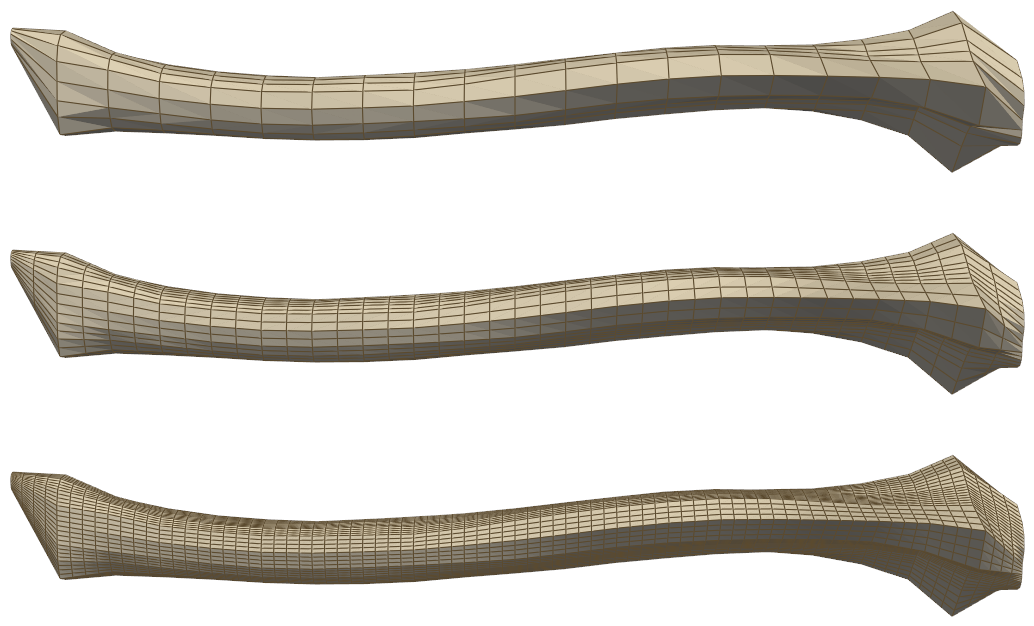
\includegraphics[width=0.92\textwidth]{images/figee_maillages.png}
  \caption{La géométrie figée maillée en C3D8 avec $k = 1$ (640 éléments, en haut), $k = 2$ (5\,120 éléments) et
  $k = 4$ (40\,960 éléments, en bas) : la forme ne change pas, seul le maillage s'affine.}
  \label{fig-figee-maillages}
\end{figure}

\subsection{Résultats}

La \cref{fig-convergence} est la courbe de convergence, en échelle linéaire comme dans les études faites avec Abaqus :
contrainte de von Mises maximale au milieu de la diaphyse en fonction du nombre de nœuds (à gauche) et du nombre
d'éléments (à droite). La \cref{fig-erreur} montre les mêmes points en échelle logarithmique et en écart au plateau.
Dans tous les calculs, la réaction à l'encastrement vaut 301,5~N, la norme de la force appliquée : l'équilibre est
respecté.

\begin{figure}[p]
  \centering
  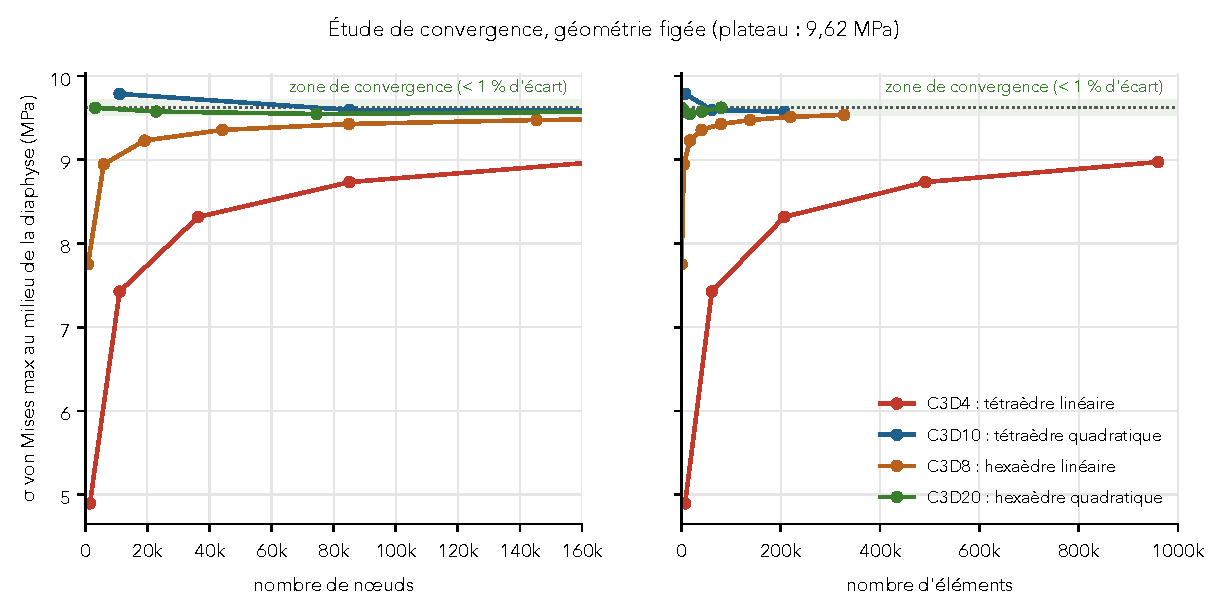
\includegraphics[width=\textwidth]{images/figee_convergence.pdf}
  \caption{Étude de convergence à géométrie figée : contrainte de von Mises maximale au milieu de la diaphyse en
  fonction du nombre de nœuds et du nombre d'éléments. La bande verte est la zone de convergence (moins de 1~\%
  d'écart au plateau, 9,62~MPa).}
  \label{fig-convergence}
  \vspace{0.6cm}
  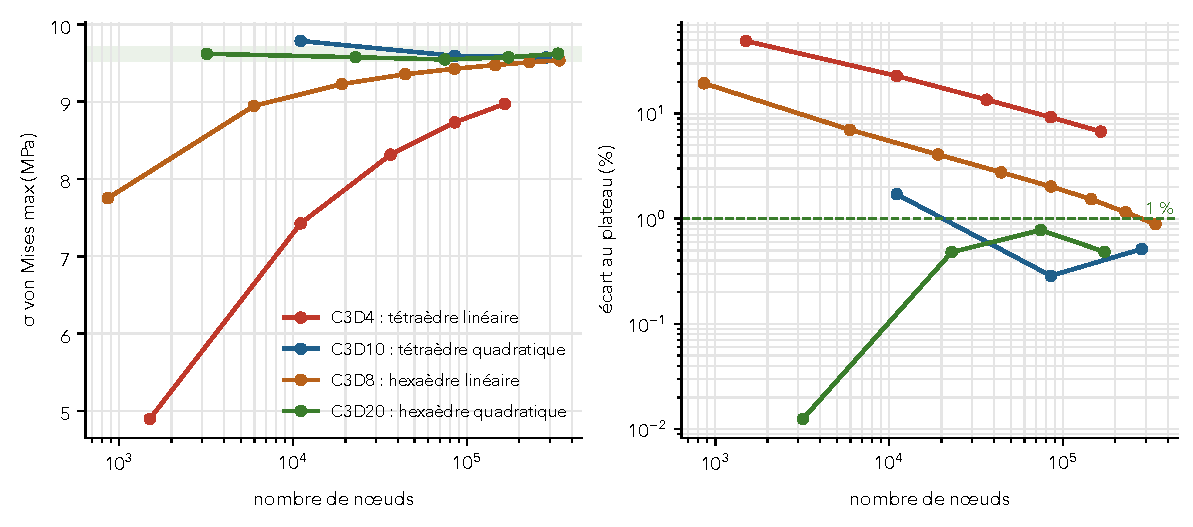
\includegraphics[width=\textwidth]{images/figee_log.pdf}
  \caption{Les mêmes résultats en échelle logarithmique (à gauche) et en écart au plateau (à droite). Le trait
  pointillé marque 1~\%.}
  \label{fig-erreur}
\end{figure}

\begin{table}[h]
\centering\small
\caption{Résumé de l'étude à géométrie figée. Plateau : 9,62~MPa (C3D20, $k = 5$).}
\label{tab-convergence}
\begin{tabular}{lrrrrl}
\toprule
\textbf{Élément} & \textbf{$k$} & \textbf{Nœuds} & \textbf{Éléments} & \textbf{$\sigma$ (MPa)} & \textbf{Écart au plateau} \\
\midrule
C3D4 & 1 & 1\,501 & 7\,680 & 4,90 & $-49$~\% \\
C3D4 & 5 & 164\,941 & 960\,000 & 8,97 & $-6{,}7$~\% \\
C3D8 & 1 & 861 & 640 & 7,75 & $-19$~\% \\
C3D8 & 8 & 340\,193 & 327\,680 & 9,54 & $-0{,}9$~\% \\
C3D10 & 1 & 11\,065 & 7\,680 & 9,79 & $+1{,}7$~\% \\
C3D10 & 3 & 283\,561 & 207\,360 & 9,57 & $-0{,}5$~\% \\
C3D20 & 1 & 3\,193 & 640 & 9,62 & $0{,}0$~\% \\
C3D20 & 5 & 334\,681 & 80\,000 & 9,62 & plateau \\
\bottomrule
\end{tabular}
\end{table}

\textbf{Lecture des résultats} :
\begin{itemize}
  \item les quatre courbes ont la forme attendue : elles se stabilisent sur le même \textbf{plateau}, environ
  9,6~MPa. Une fois le plateau atteint, ajouter des nœuds ne change plus le résultat : le maillage est assez fin ;
  \item les éléments \textbf{linéaires} y arrivent \emph{par en dessous}. Le \textbf{C3D8} part de 7,75~MPa
  (640 éléments, $-19$~\%), dépasse 9,2~MPa dès 19\,000 nœuds et entre dans la zone des 1~\% vers 340\,000 nœuds. Le
  \textbf{C3D4} part de beaucoup plus bas (4,9~MPa, $-49$~\%) et reste à $-6{,}7$~\% avec 165\,000 nœuds : c'est le
  verrouillage vu sur la poutre, un élément à déformation constante est trop raide en flexion ;
  \item les éléments \textbf{quadratiques} sont presque sur le plateau dès le premier maillage : le \textbf{C3D20}
  est à moins de 1~\% partout, avec seulement 640 éléments ; le \textbf{C3D10} arrive \emph{par au-dessus} (+1,7~\% avec
  7\,680 éléments) et entre dans la zone des 1~\% dès $k = 2$. Leur contrainte varie linéairement dans l'élément, ce
  qui suffit à représenter la flexion ;
  \item à précision égale, les quadratiques demandent beaucoup moins de nœuds : 1~\% d'écart avec 3\,000 nœuds en
  C3D20, contre plus de 300\,000 en C3D8 ;
  \item ordre de convergence : quand la taille des éléments est divisée par 2 ($k$ doublé, nombre de nœuds multiplié
  par 8 environ), l'écart du C3D8 passe de 19~\% à 7~\%, puis 2,8~\% et 0,9~\% : il est divisé par 2,5 à 3 à chaque
  fois. L'erreur décroît donc comme $h^{p}$ avec $p \approx 1{,}5$ ($2^{1{,}5} \approx 2{,}8$), un peu plus vite que
  l'ordre 1 attendu pour la contrainte d'un élément linéaire (la moyenne des contraintes aux nœuds aide).
\end{itemize}

\subsection{La force ne change pas le nombre de nœuds nécessaire}
\label{sec-force}

On pourrait penser qu'une force plus faible demande moins de nœuds. Ce n'est pas le cas en élasticité linéaire : le
déplacement et la contrainte sont \emph{proportionnels} à la force ($\vb{K}\vb{u} = \vb{f}$, donc $\vb{u}$ double quand
$\vb{f}$ double), et le nombre de nœuds est fixé par le maillage, pas par la charge. La série C3D8 a été refaite avec la
moitié et le double de la force (\cref{fig-force}) : toutes les contraintes sont exactement divisées ou multipliées par 2
(par exemple 3,876, 7,752 et 15,505~MPa pour $k = 1$), et le plateau est atteint au même nombre de nœuds. Ramenées à
la même force, les trois courbes se superposent. La force change donc la \emph{hauteur} du plateau, pas l'endroit où on
l'atteint. (Ce ne serait plus vrai avec un calcul non linéaire : plasticité, grands déplacements ou contact.)

\begin{figure}[h]
  \centering
  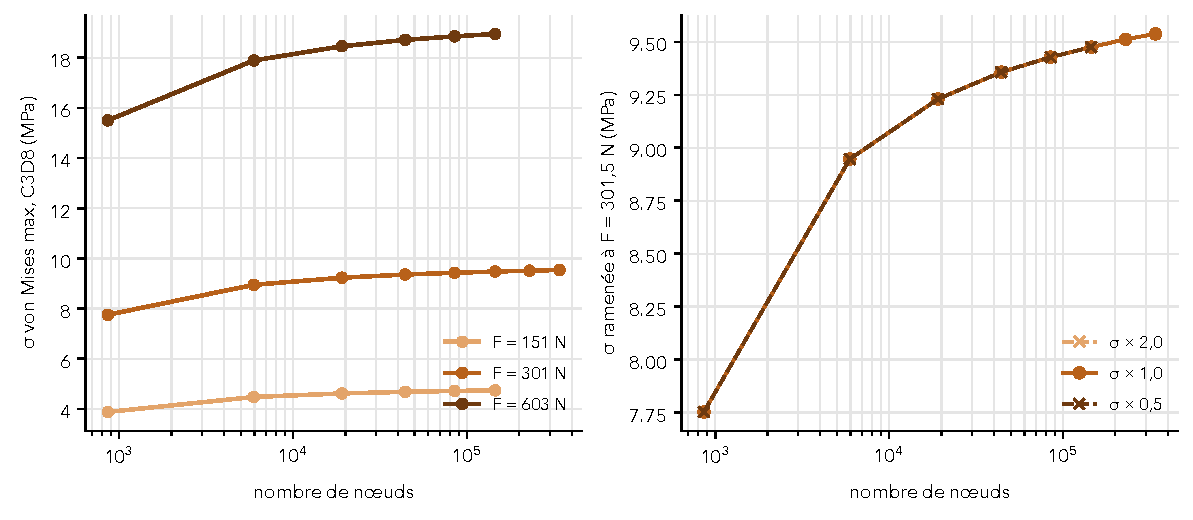
\includegraphics[width=\textwidth]{images/figee_force.pdf}
  \caption{Série C3D8 avec trois forces (151, 301 et 603~N) : les contraintes sont proportionnelles à la force (à
  gauche) ; ramenées à 301,5~N, les trois courbes se superposent (à droite).}
  \label{fig-force}
\end{figure}

\subsection{Avec des maillages libres qui suivent l'os}
\label{sec-libres}

Avant l'étude à géométrie figée, nous avons fait une première étude où chaque maillage suivait le STL de plus près.
Elle est moins propre (la géométrie change avec la taille des éléments), mais elle montre trois pièges utiles. Trois
familles de maillages ont été comparées (\cref{fig-maillages}) :
\begin{itemize}
  \item \textbf{tétraèdres} (C3D4, C3D10) : surface du STL remaillée en triangles réguliers de taille $h$ (pyacvd),
  puis TetGen remplit le volume ;
  \item \textbf{hexaèdres balayés} (C3D8, C3D20) : l'os est coupé en tranches perpendiculaires à son axe, et chaque
  section est maillée par la même grille en « O » (un carré au centre, des couronnes qui rejoignent le contour,
  \cref{fig-section-o}), comme un maillage \emph{sweep} d'Abaqus ;
  \item \textbf{hexaèdres voxels} : des cubes de côté $h$ dont le centre est dans l'os (surface en escalier).
\end{itemize}

\begin{figure}[h]
  \centering
  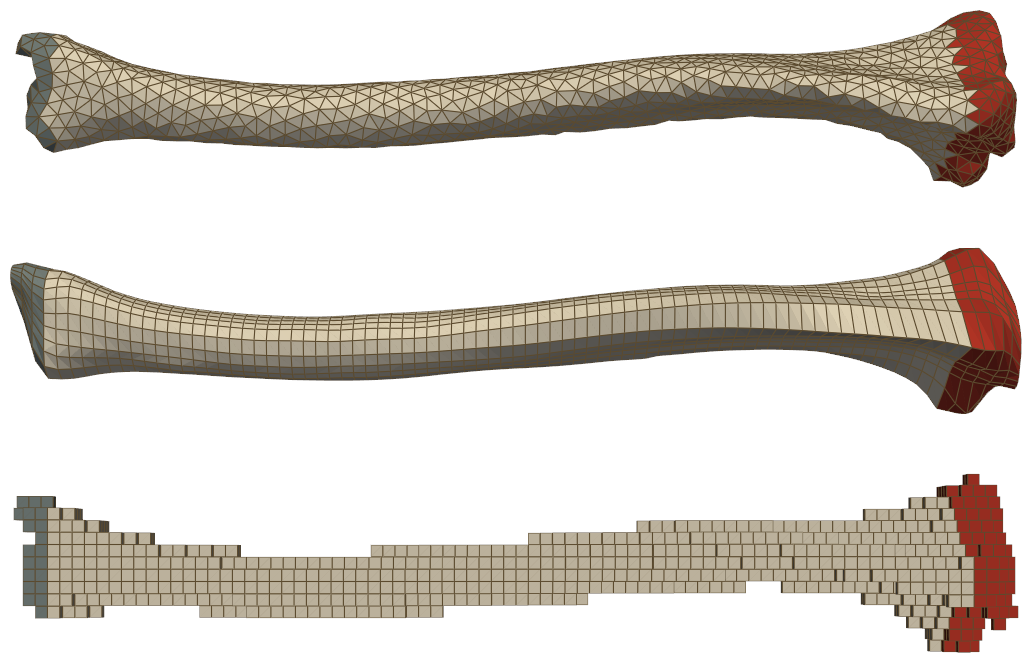
\includegraphics[width=\textwidth]{images/maillages_tibia.png}
  \caption{Les trois familles de maillages libres : tétraèdres TetGen ($h = 4$~mm, en haut), hexaèdres balayés
  ($h = 3$~mm, au milieu), hexaèdres voxels ($h = 3$~mm, en bas). En gris : la zone encastrée (cheville) ; en rouge :
  la zone chargée (genou).}
  \label{fig-maillages}
\end{figure}

\begin{figure}[h]
  \centering
  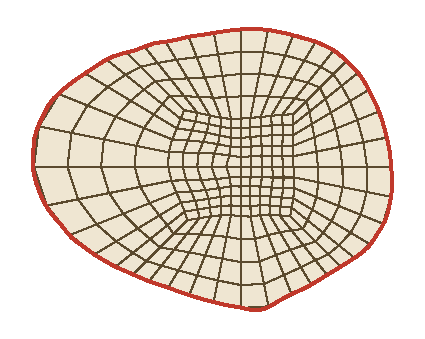
\includegraphics[width=0.36\textwidth]{images/section_o.pdf}
  \caption{Une section du maillage balayé au milieu de la diaphyse ($h = 1{,}6$~mm) : la grille en « O » épouse le
  contour réel de l'os (en rouge).}
  \label{fig-section-o}
\end{figure}

Les tétraèdres et les hexaèdres balayés convergent vers $8{,}8 \pm 0{,}1$~MPa (\cref{fig-libre}). C'est moins que les
9,6~MPa de la géométrie figée, parce que la vraie section de l'os est plus grande que celle du tibia simplifié. Les
C3D10 oscillent de $\pm 1$~\% d'un maillage à l'autre : TetGen refait à chaque fois un maillage différent, non emboîté
dans le précédent. C'est la raison pour laquelle l'étude principale utilise une géométrie figée.

\begin{figure}[h]
  \centering
  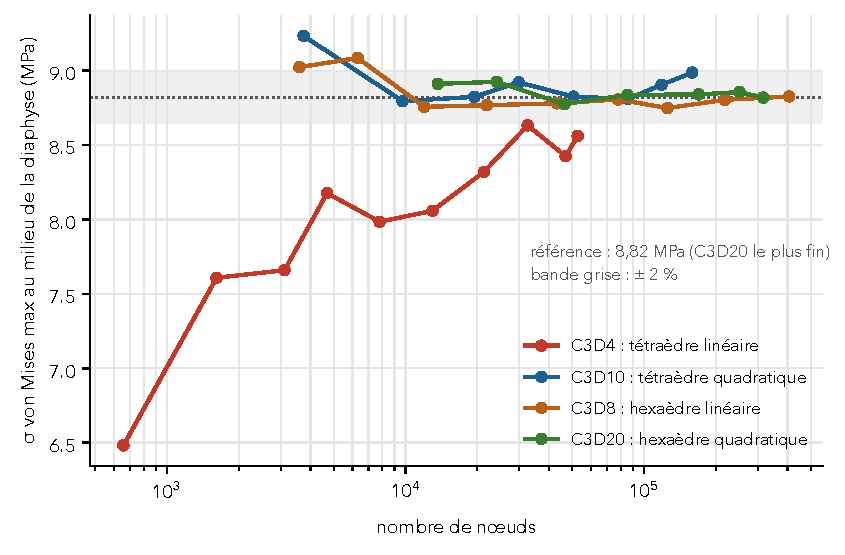
\includegraphics[width=0.95\textwidth]{images/libre_milieu.pdf}
  \caption{Maillages libres : contrainte au milieu de la diaphyse en fonction du nombre de nœuds (bande grise :
  ± 2~\% autour du C3D20 le plus fin, 8,82~MPa).}
  \label{fig-libre}
\end{figure}

\subsubsection{Piège 1 : les nœuds milieux doivent être sur la surface}

Avec une géométrie qui change, un élément quadratique dont les nœuds milieux sont au milieu d'arêtes droites garde une
surface facettée : la section est un peu trop petite et la contrainte un peu trop forte. Abaqus place les nœuds
milieux des arêtes de surface sur la géométrie ; nous faisons de même (projection sur le STL, ou même transformation
que les sommets pour le maillage balayé), sauf pour un élément dont le jacobien varierait trop (rapport minimum sur
maximum sous 0,3). Avec $h = 4$~mm, l'écart passe de 7,5~\% à 1~\% pour le C3D20, et de 4,8~\% à 0,3~\% pour le C3D10
(\cref{fig-courbes}).

\begin{figure}[h]
  \centering
  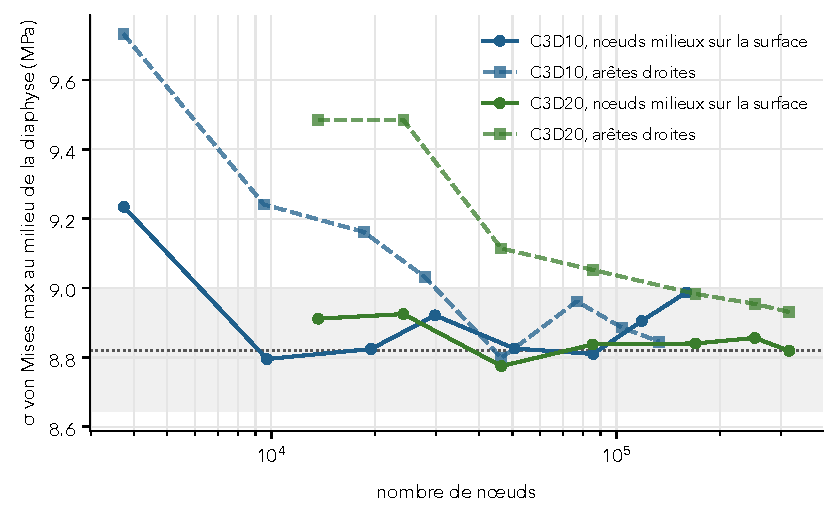
\includegraphics[width=0.95\textwidth]{images/libre_courbes.pdf}
  \caption{Maillages libres, éléments quadratiques : nœuds milieux sur la surface courbe de l'os (traits pleins) ou
  au milieu d'arêtes droites (tirets).}
  \label{fig-courbes}
\end{figure}

\subsubsection{Piège 2 : les voxels ne convergent pas pour une contrainte de surface}

Les hexaèdres voxels donnent des déplacements corrects, mais une contrainte au milieu de la diaphyse trop forte (10 à
12~MPa), qui ne converge pas (\cref{fig-voxels}). Chaque marche de l'escalier est un petit coin rentrant où la
contrainte se concentre ; quand on raffine, les marches deviennent plus petites mais plus nombreuses, et le pic ne
disparaît pas. Pour une contrainte à la surface de l'os, il faut un maillage qui suit la surface.

\begin{figure}[h]
  \centering
  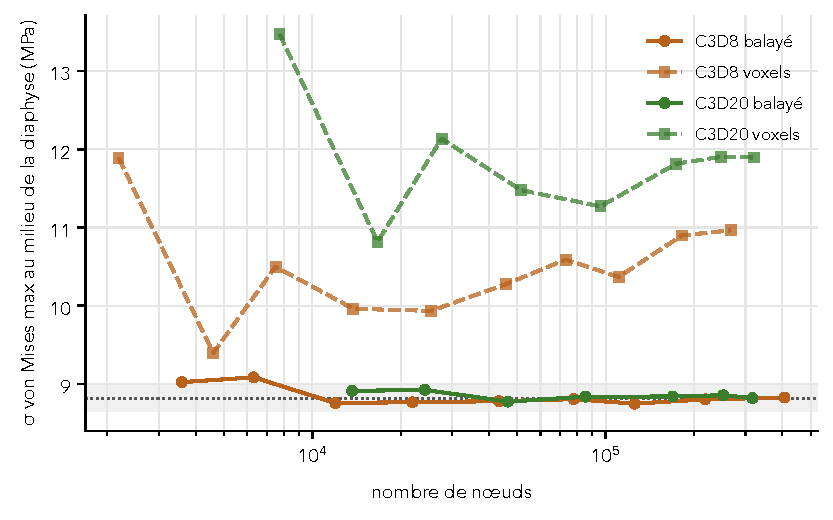
\includegraphics[width=0.95\textwidth]{images/libre_voxels.pdf}
  \caption{Hexaèdres : maillage balayé qui suit la surface (traits pleins) contre voxels en escalier (tirets).}
  \label{fig-voxels}
\end{figure}

\subsubsection{Piège 3 : le maximum sur tout l'os ne converge pas}

Si l'on suit la contrainte maximale sur \emph{tout} l'os au lieu du milieu de la diaphyse, la courbe ne se stabilise
pas (\cref{fig-max}) : avec les C3D10, elle saute d'un maillage à l'autre, de 12 à 36~MPa. Ce maximum est au bord de
la zone encastrée, là où un nœud bloqué touche un nœud libre. En élasticité, la contrainte y est théoriquement infinie
(une \emph{singularité}) : la valeur calculée dépend de la taille et de la forme du plus petit élément qui touche ce
bord. Ce n'est pas un défaut du maillage mais du modèle (un encastrement parfait n'existe pas). Il ne faut jamais faire
une étude de convergence sur un tel point : on choisit une zone loin des appuis et des charges.

\begin{figure}[h]
  \centering
  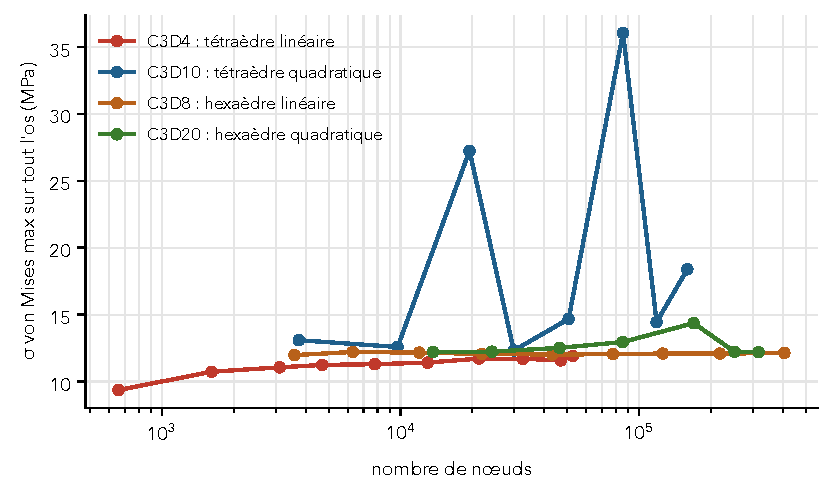
\includegraphics[width=0.95\textwidth]{images/libre_max.pdf}
  \caption{Contrainte maximale sur tout l'os : elle ne converge pas (singularité au bord de l'encastrement).}
  \label{fig-max}
\end{figure}

\subsection{Refaire l'étude dans Abaqus}

Le dossier \fichier{etude\_convergence/abaqus/} contient un fichier \fichier{.inp} par maillage de l'étude à
géométrie figée (par exemple \fichier{tibia\_figee\_C3D8\_k3.inp}). Chaque fichier est complet : nœuds, éléments,
matériau, ensembles \texttt{ENCASTREMENT} (nœuds), \texttt{CHARGE} et \texttt{MILIEU} (éléments), charge volumique
(\texttt{*Dload}, \texttt{BX}, \texttt{BY}, \texttt{BZ}) et un pas statique. Il s'ouvre dans Abaqus/CAE (File, Import,
Model) ou se lance directement (\texttt{abaqus job=tibia\_figee\_C3D8\_k3 interactive}). Dans le module
Visualization, on affiche S, Mises et on relève le maximum sur l'ensemble \texttt{MILIEU}, puis on reporte la valeur
en fonction du nombre de nœuds.

Pour tester l'élément hexaédrique par défaut d'Abaqus, le \textbf{C3D8R} (intégration réduite à un point, avec
contrôle du « hourglass »), il suffit de remplacer \texttt{type=C3D8} par \texttt{type=C3D8R} dans la ligne
\texttt{*Element} du fichier (de même \texttt{C3D20R}). Cet élément n'est pas programmé dans notre code, car son
contrôle du hourglass est propre à Abaqus. Il est en général moins raide en flexion que le C3D8 et atteint le
plateau plus vite. Les fichiers \fichier{.inp} n'ont pas pu être testés dans Abaqus : leur format suit le manuel, et
le même maillage est résolu par notre code. Le script \fichier{etude\_convergence.py --inp} écrit aussi ceux des
maillages libres.


% ================================================================================================ 9
\section{Limites et pistes d'amélioration}
\label{sec-limites}

\subsection{Ce qui n'est pas encore validé}

\begin{itemize}
  \item \textbf{Pas de vérité terrain sur un vrai os.} L'exactitude est mesurée sur un faux scanner ; sur le
  lévrier, nous mesurons seulement la stabilité (sensibilité au seuil). Une validation solide comparerait nos
  segmentations à des segmentations faites à la main par un expert (par exemple dans 3D Slicer), avec des mesures
  classiques : le \textbf{coefficient de Dice} $2|A \cap B| / (|A| + |B|)$ pour le recouvrement des volumes, et la
  \textbf{distance de Hausdorff} (ou son 95\textsuperscript{e} centile) pour l'écart entre les surfaces. Un os imprimé ou
  un os sec scanné puis mesuré au pied à coulisse donnerait aussi une référence physique.
  \item \textbf{Un seul animal, un seul scanner.} Les réglages (taille minimale des graines, persistance, seuil de
  $c^*$) ont été ajustés sur trois séries d'un même lévrier. D'autres races, d'autres scanners ou d'autres noyaux de
  reconstruction peuvent demander de les revoir.
\end{itemize}

\subsection{Limites de la méthode}

\begin{itemize}
  \item \textbf{Seuil global.} Le seuil de 226~HU est le même pour tout le volume. Un os peu dense (animal âgé,
  ostéoporose, jeune animal avec des cartilages de croissance) ou un scanner mal calibré peut donner des trous. Un
  seuil adapté à chaque série, déduit de l'histogramme des HU, serait une amélioration simple.
  \item \textbf{Interlignes très fins.} Quand l'interligne est plus fin que le flou du scanner (coude, petits os du
  tarse), la frontière entre deux os peut être mal placée. Le lissage de frontière limite le problème sans le
  supprimer.
  \item \textbf{Règles anatomiques spécifiques.} L'identification repose sur des règles écrites pour le membre
  pelvien du chien (et, en partie, le membre thoracique). Elles ne s'appliquent pas telles quelles à une autre espèce
  ou à une autre région du corps. Une fracture ou une forte déformation peut aussi tromper les règles de forme.
  \item \textbf{Métal.} Une plaque ou des vis créent des artefacts (stries très denses) que la méthode ne traite pas.
  \item \textbf{Cartilage.} Le scanner ne voit pas le cartilage : la surface articulaire du STL est celle de l'os
  sous-chondral.
\end{itemize}

\subsection{Pistes pour aller plus loin}

\begin{itemize}
  \item Construire un petit jeu de segmentations manuelles de référence et calculer Dice et Hausdorff pour chaque
  os.
  \item Comparer notre méthode à des outils existants : les outils de seuillage et de « Grow from seeds » de 3D Slicer,
  ou des réseaux de neurones de segmentation (famille U-Net). Ces réseaux sont très performants, mais demandent des
  centaines de cas annotés ; notre méthode, elle, n'a besoin d'aucun apprentissage.
  \item Choisir le seuil automatiquement (histogramme, méthode d'Otsu) et mesurer l'effet sur la sensibilité.
  \item Remplacer le seuil de $c^*$ fixe par une décision apprise sur plusieurs animaux.
\end{itemize}

% ================================================================================================ 10
\section{Utiliser le module}
\label{sec-utiliser}

\subsection{Installation}

Il faut Python 3.10 ou plus récent et les bibliothèques numpy, scipy, pydicom, SimpleITK, VTK, trimesh, pyvista et
matplotlib (liste complète : \fichier{application/requirements.txt}).

\begin{Verbatim}
python -m venv .venv
.venv/bin/pip install -r application/requirements.txt
\end{Verbatim}

\subsection{En ligne de commande}

Le script \fichier{lancer\_tout.py} enchaîne toutes les étapes du projet (y compris l'étape 6, les repères) :

\begin{Verbatim}
cd code_source
python lancer_tout.py --liste                  # séries trouvées dans ../dicom
python lancer_tout.py --serie knee_to_ankle    # une série (un morceau de nom suffit)
python lancer_tout.py --dossier "D:/scanner" --sortie "D:/resultats" --seuil 250 --ras
python tests/test_chaine.py                    # test sur le faux scanner (2 s)
\end{Verbatim}

Options utiles : \texttt{--seuil} change le seuil de l'os, \texttt{--ras} écrit les STL en RAS,
\texttt{--sans-controle} saute la sensibilité au seuil, \texttt{--sans-images} saute les aperçus.

\subsection{Depuis Python, étapes 1 à 5 seulement}

Pour utiliser le module seul, sans la partie chirurgicale, on appelle directement les cinq étapes. Ce code a été
exécuté le 23/11/2026 sur la série genou et cheville (30~s, résultats identiques à ceux du dossier \fichier{exemples/}) :

\begin{Verbatim}
import time
import etape1_lecture_dicom as E1, etape2_segmentation as E2
import etape3_identification as E3, etape4_maillage as E4, etape5_controle as E5

debut = time.time()
serie = E1.trouver(E1.inventaire("../dicom/Greyhound hindlimb knee to ankle"), "knee")
volume = E1.charger(serie)                 # étape 1 : volume en HU + matrice A
seg = E2.segmenter(volume)                 # étape 2 : étiquettes
E3.identifier(seg)                         # étape 3 : noms et corrections
bilan = E4.exporter(seg, "sortie")         # étape 4 : un STL par os + seg.nrrd
E5.controler(seg, volume, bilan, "sortie", debut)   # étape 5 : rapports
\end{Verbatim}

\subsection{Corriger avec des points nommés}
\label{sec-graines-json}

Si un os est mal reconnu ou si deux os restent collés, on place un ou plusieurs points nommés dans le fichier
\fichier{resultats/<série>/graines.json} (l'application le fait par un clic), puis on relance le calcul :

\begin{Verbatim}
{"points": [
  {"nom": "femur", "position": [18.0, -41.0, -150.0], "systeme": "LPS"},
  {"nom": "tibia", "position": [20.5, -38.2, -260.0], "systeme": "LPS"}
]}
\end{Verbatim}

\subsection{Vérifier dans 3D Slicer}

Dans 3D Slicer : charger la série DICOM, puis glisser \fichier{segmentation.seg.nrrd} dans la fenêtre. Chaque os
apparaît comme un segment nommé et coloré, superposé aux coupes. Les STL peuvent aussi être glissés directement : en
LPS, ils tombent exactement sur l'image (3D Slicer, depuis la version 4.11, lit et écrit les modèles en LPS par
défaut).

% ================================================================================================ annexes
\clearpage
\appendix
\section{Les paramètres}
\label{ann-parametres}

Tous les réglages sont dans \fichier{code\_source/parametres.py}. Aucun autre nombre « magique » n'apparaît dans le
code.

\begin{longtable}{p{5.6cm}rp{7.4cm}}
\toprule
\textbf{Paramètre} & \textbf{Valeur} & \textbf{Rôle et origine} \\
\midrule
\endhead
\multicolumn{3}{l}{\textit{Étape 1 : lecture}} \\
\texttt{EPAISSEUR\_MAX\_MM} & 1,0 & coupes plus épaisses : avertissement (cahier des charges) \\
\texttt{TOLERANCE\_ESPACEMENT} & 0,05 & écart relatif toléré entre deux intervalles de coupes \\
\texttt{TOLERANCE\_ORIENTATION} & 0,001 & cosinus directeurs identiques à cette précision \\
\multicolumn{3}{l}{\textit{Étape 2 : segmentation}} \\
\texttt{SIGMA\_LISSAGE\_MM} & 0,35 & flou gaussien ; divise le bruit (49~HU) environ par deux \\
\texttt{SEUIL\_OS\_HU} & 226 & masque osseux (seuil « Bone » de Mimics) \\
\texttt{MARGE\_RECADRAGE\_MM} & 6 & marge autour des os denses \\
\texttt{SEUIL\_GRAINE\_DEPART\_HU} & 500 & premier palier des graines \\
\texttt{SEUIL\_GRAINE\_MAX\_HU} & 1500 & dernier palier \\
\texttt{PAS\_SEUIL\_HU} & 100 & pas entre paliers \\
\texttt{VOLUME\_MIN\_MORCEAU\_MM3} & 300 & taille minimale d'un morceau pour devenir une graine \\
\texttt{PERSISTANCE\_HU} & 200 & un morceau doit exister encore 200~HU plus haut\ldots \\
\texttt{VOLUME\_PERSISTANCE\_MM3} & 50 & \ldots{} avec au moins ce volume \\
\texttt{VOLUME\_MIN\_GRAINE\_MM3} & 30 & bloc dense plus petit : pas de graine \\
\texttt{VOLUME\_MIN\_SEGMENT\_MM3} & 50 & segment plus petit : rattaché au voisin \\
\texttt{RAPPORT\_CONTACT\_FUSION} & 3,0 & recollage si $c^* \geq 3$ (mesuré : coupure 5, articulation ≤ 2,1) \\
\multicolumn{3}{l}{\textit{Étape 3 : identification}} \\
\texttt{LONGUEUR\_OS\_LONG\_MM} & 50 & os long : au moins 50~mm\ldots \\
\texttt{ALLONGEMENT\_OS\_LONG} & 3,0 & \ldots{} et allongement au moins 3 \\
\texttt{ALLONGEMENT\_COMPACT} & 3,5 & os compact (tarse, patella) \\
\texttt{CV\_MAX\_OBJET} & 0,2 & objet non osseux : densité homogène\ldots \\
\texttt{FRACTION\_SPONGIEUX\_MAX\_OBJET} & 0,08 & \ldots{} presque pas de voxels sous 600~HU\ldots \\
\texttt{CAVITE\_MAX\_OBJET} & 0,05 & \ldots{} et pas de cavité \\
\texttt{RAYON\_VALLEE\_MM} & 1,0 & taille de l'interligne cherché (chapeau haut-de-forme noir) \\
\texttt{PROFONDEUR\_VALLEE\_HU} & 250 & profondeur minimale de la vallée \\
\texttt{RAYON\_TETE\_MM} & 4 à 20 & rayon plausible d'une tête fémorale de chien \\
\texttt{TOLERANCE\_SPHERE\_MM} & 0,6 & distance d'un point à la sphère \\
\texttt{COUVERTURE\_MIN\_SPHERE} & 0,4 & fraction des directions couvertes (lévrier : 69~\%) \\
\texttt{INLIERS\_MIN\_SPHERE} & 150 & points minimum sur la sphère (lévrier : 2055) \\
\texttt{PAS\_TRANCHES\_MM} & 2,0 & tranches pour trouver la fibula \\
\texttt{RAPPORT\_AIRE\_FIBULA\_MAX} & 0,2 & aire de la fibula / aire du tibia \\
\texttt{RAYON\_GRAINE\_MM} & 2,5 & boule autour d'un point de l'utilisateur \\
\multicolumn{3}{l}{\textit{Étape 4 : maillage}} \\
\texttt{RAYON\_FERMETURE\_MM} & 1,0 & fermeture avant remplissage \\
\texttt{SIGMA\_MAILLAGE\_MM} & 0,3 & flou du masque avant marching cubes \\
\texttt{ITERATIONS\_LISSAGE} & 20 & lissage windowed sinc\ldots \\
\texttt{BANDE\_PASSANTE\_LISSAGE} & 0,05 & \ldots{} et sa bande passante \\
\texttt{TRIANGLES\_MAX} & 150\,000 & décimation au-delà \\
\texttt{REDUCTION\_MAX} & 0,75 & jamais plus de 75~\% des triangles retirés \\
\texttt{AFFINAGE\_DEMI\_HAUTEUR} & oui & correction du biais du seuil bas \\
\texttt{PROFIL\_INTERIEUR\_MM} & 2,5 & profil lu de 2,5~mm dans l'os\ldots \\
\texttt{PROFIL\_EXTERIEUR\_MM} & 2,0 & \ldots{} à 2~mm dehors \\
\texttt{CONTRASTE\_MIN\_HU} & 300 & contraste minimal pour faire confiance au profil \\
\texttt{DEPLACEMENT\_MAX\_MM} & 1,5 & déplacement maximal d'un sommet \\
\texttt{LISSAGE\_DEPLACEMENT} & 5 & passes de moyenne des déplacements \\
\texttt{SYSTEME\_COORDONNEES} & LPS & repère des STL (ou RAS) \\
\multicolumn{3}{l}{\textit{Étape 5 : contrôle}} \\
\texttt{VARIATION\_SEUIL\_HU} & 50 & variation du seuil (cahier des charges) \\
\texttt{ECART\_SURFACE\_CIBLE\_MM} & 0,5 & objectif d'écart entre surfaces \\
\bottomrule
\end{longtable}

\section{Où trouver chaque chose dans le code}
\label{ann-code}

\begin{longtable}{p{4.2cm}p{11cm}}
\toprule
\textbf{Fichier} & \textbf{Fonctions principales} \\
\midrule
\endhead
\fichier{etape1\_lecture\_dicom.py} & \texttt{inventaire} (séries d'un dossier), \texttt{charger} (tri, contrôles, HU,
matrice $\vb{A}$), \texttt{trouver} (série par son nom) ; classes \texttt{Serie} et \texttt{Volume} \\
\fichier{etape2\_segmentation.py} & \texttt{segmenter} (enchaîne tout), \texttt{recadrage}, \texttt{lisser},
\texttt{graines\_automatiques} (arbre des seuils), \texttt{croissance} (ligne de partage des eaux),
\texttt{contacts}, \texttt{fusionner\_surdecoupages} (critère $c^*$), \texttt{nettoyer} ; outils :
\texttt{recroissance}, \texttt{raffiner}, \texttt{lisser\_frontiere}, \texttt{boule} ; classe \texttt{Segmentation} \\
\fichier{etape3\_identification.py} & \texttt{identifier} (toutes les règles, dans l'ordre), \texttt{decrire}
(descripteurs), \texttt{tete\_femorale} et \texttt{ajuster\_sphere} (RANSAC), \texttt{separer\_fibula},
\texttt{membre\_thoracique}, \texttt{separer\_par\_points}, \texttt{nettoyer\_morceaux}, \texttt{nommer\_cotes} \\
\fichier{etape4\_maillage.py} & \texttt{exporter} (tous les os d'une série), \texttt{mailler} (un os),
\texttt{remplir}, \texttt{affiner\_demi\_hauteur}, \texttt{controle} (étanchéité, Euler), \texttt{bords\_touches},
\texttt{ecrire\_stl}, \texttt{ecrire\_seg\_nrrd}, \texttt{lire\_seg\_nrrd} \\
\fichier{etape5\_controle.py} & \texttt{controler} (tout), \texttt{sensibilite\_seuil}, \texttt{apercu\_3d},
\texttt{apercu\_coupes}, \texttt{rapport\_md}, \texttt{markups} \\
\fichier{parametres.py} & tous les réglages (\cref{ann-parametres}) \\
\fichier{lancer\_tout.py} & la ligne de commande \\
\fichier{tests/test\_chaine.py} & le faux scanner et ses 14 vérifications \\
\fichier{etude\_convergence/ef.py} & éléments C3D4, C3D10, C3D8, C3D20 : \texttt{ELEMENTS}, \texttt{assembler},
\texttt{resoudre}, \texttt{contraintes\_noeuds}, \texttt{ecrire\_inp} (fichier Abaqus) \\
\fichier{etude\_convergence/maillages.py} & \texttt{tetraedres} (TetGen), \texttt{balaye} (grille en « O »),
\texttt{voxels}, \texttt{quadratique} (nœuds milieux) \\
\fichier{etude\_convergence/etude\_convergence.py} & l'étude de convergence et ses figures \\
\bottomrule
\end{longtable}

\section{Petit glossaire}

\begin{description}[style=nextline, leftmargin=1.2cm, itemsep=1pt]
  \item[ACP] analyse en composantes principales : trouve les directions principales d'un nuage de points.
  \item[Composante connexe] groupe de voxels qui se touchent (ici par une face, une arête ou un coin).
  \item[Convergence (étude de)] refaire un calcul avec des maillages de plus en plus fins jusqu'à ce que le résultat ne
  change plus.
  \item[DICOM] format standard des images médicales : une coupe par fichier, avec un en-tête (patient, géométrie).
  \item[Étanche] se dit d'un maillage fermé, sans trou, dont chaque arête est partagée par deux triangles.
  \item[Élément quadratique] élément fini avec un nœud au milieu de chaque arête : le déplacement y varie comme un
  polynôme de degré 2 (C3D10, C3D20).
  \item[Fermeture morphologique] dilatation suivie d'une érosion : bouche les petits trous et les fentes étroites.
  \item[Graine] petit groupe de voxels dont on est sûr qu'il appartient à un os donné ; point de départ de la croissance.
  \item[HU] unité Hounsfield : échelle des valeurs du scanner (eau 0, air $-1000$).
  \item[Interligne] espace entre deux os d'une articulation, rempli de cartilage et de liquide (peu dense).
  \item[LPS, RAS] repères du patient : gauche, arrière, haut (DICOM) ou droite, avant, haut (3D Slicer).
  \item[Marching cubes] algorithme qui extrait une surface de triangles d'une image 3D.
  \item[RANSAC] méthode d'ajustement robuste : on tire au hasard le minimum de points, on garde le modèle qui
  explique le plus de points.
  \item[Maillage balayé] maillage hexaédrique obtenu en répétant le maillage d'une section le long d'un axe
  (« sweep » dans Abaqus).
  \item[Segmentation] attribution d'une étiquette (un os) à chaque voxel.
  \item[Singularité] point où la contrainte calculée augmente sans fin quand on raffine (coin rentrant, bord d'un
  encastrement).
  \item[STL] format de fichier qui liste les triangles d'une surface.
  \item[Verrouillage] raideur artificielle d'un élément qui ne sait pas représenter la déformation (C3D4 en flexion).
  \item[Volume partiel] un voxel à cheval sur deux tissus prend une valeur intermédiaire.
  \item[Voxel] petit pavé élémentaire du volume, l'équivalent 3D du pixel.
\end{description}

% ================================================================================================ références
\begin{thebibliography}{99}
\bibitem{fedorov2012} Fedorov A, Beichel R, Kalpathy-Cramer J, et al. 3D Slicer as an image computing platform for
the Quantitative Imaging Network. \emph{Magnetic Resonance Imaging} 2012;30(9):1323-1341.
\bibitem{fischler1981} Fischler MA, Bolles RC. Random sample consensus: a paradigm for model fitting with applications
to image analysis and automated cartography. \emph{Communications of the ACM} 1981;24(6):381-395.
\bibitem{garland1997} Garland M, Heckbert PS. Surface simplification using quadric error metrics. \emph{Proceedings
of SIGGRAPH '97}, 1997:209-216.
\bibitem{lorensen1987} Lorensen WE, Cline HE. Marching cubes: a high resolution 3D surface construction algorithm.
\emph{Computer Graphics (SIGGRAPH '87)} 1987;21(4):163-169.
\bibitem{lowekamp2013} Lowekamp BC, Chen DT, Ibáñez L, Blezek D. The design of SimpleITK. \emph{Frontiers in
Neuroinformatics} 2013;7:45.
\bibitem{maurer2003} Maurer CR, Qi R, Raghavan V. A linear time algorithm for computing exact Euclidean distance
transforms of binary images in arbitrary dimensions. \emph{IEEE Transactions on Pattern Analysis and Machine
Intelligence} 2003;25(2):265-270.
\bibitem{meyer1994} Meyer F. Topographic distance and watershed lines. \emph{Signal Processing} 1994;38(1):113-125.
\bibitem{schroeder2015} Schroeder W, Maynard R, Geveci B. Flying edges: a high-performance scalable isocontouring
algorithm. \emph{IEEE Symposium on Large Data Analysis and Visualization (LDAV)}, 2015.
\bibitem{taubin1995} Taubin G. A signal processing approach to fair surface design. \emph{Proceedings of SIGGRAPH
'95}, 1995:351-358.
\end{thebibliography}

\end{document}
